\documentclass[10pt, oneside]{book}
\usepackage[utf8]{inputenc}
\usepackage{amsmath}
\usepackage{amsthm}
\usepackage{amssymb}
\usepackage{enumitem}
\usepackage{mdframed}
\usepackage{hyperref}
\usepackage{systeme}
%\usepackage{moresize}
\usepackage{relsize}
\usepackage{comment}
\usepackage{cancel}
\usepackage[a4paper,left=2.3cm, right=2.3cm, top=2.1cm, bottom=2.1cm]{geometry}
\usepackage[italian]{babel}
\usepackage{ragged2e}
\usepackage{fancyhdr}
\usepackage[Lenny]{fncychap}
%\ChTitleVar{\raggedleft\Huge\bfseries\fontfamily{cmss}\selectfont}
\usepackage{tikz}
\usepackage{pgfplots}
\usetikzlibrary{decorations.pathreplacing,calligraphy}
\usetikzlibrary { decorations.pathmorphing, decorations.shapes, }
\usepackage[cal=dutchcal]{mathalfa}
\usepackage{wrapfig}
\usepackage{physics}
\usepackage{listings}
\usepackage{graphicx}
\usepackage{eso-pic, transparent}
\usetikzlibrary{calc}
\usetikzlibrary{positioning}
\pgfplotsset{width=10cm,compat= newest}
\usepgfplotslibrary{external}
%\tikzexternalize
\usepackage{bbold}
\swapnumbers
\hypersetup{
    colorlinks=true,
    linkcolor=blue,
}
 
\renewcommand{\arraystretch}{1.2}
\setlength{\tabcolsep}{0.5cm}

\renewcommand{\qedsymbol}{\hfill \large $\blacksquare$}
%\renewcommand{\descriptionlabel}{$\ast$}
\newcommand{\celsius}{\, \mathrm{{}^\circ C}}
\newcommand{\evolt}{\, \mathrm{eV}}
\newcommand{\kelvin}[1]{\, \mathrm{K^{#1}}}
\newcommand{\joule}[1]{\, \mathrm{J^{#1}}}
\newcommand{\pascal}[1]{\, \mathrm{Pa^{#1}}}
\newcommand{\molvol}{\mathrm{v}}
\newcommand{\molms}{\mathcal{M}}
\newcommand{\angstrom}{\, \mathrm{\AA}}
\newcommand{\meters}[2]{\, \mathrm{#2 m^{#1}}}
\newcommand{\grams}[1]{\, \mathrm{g^{#1}}}
\newcommand{\mols}[1]{\, \mathrm{mol^{#1}}}
\newcommand{\limit}[2]{\lim\limits_{#1 \rightarrow #2}}
\newcommand{\mean}[1]{\langle #1 \rangle}
\newcommand{\infobox}[2]{\vspace{0.5cm}~\\ \textbf{#1} \hrulefill \vspace{0.2cm}\\#2 \\\hrule \vspace{0.5cm}}
\newcommand{\lawbox}[2]{\begin{center}
\framebox{
\parbox{\linewidth}{
\vspace{0.3cm}
\textbf{#1} \hfill $\displaystyle #2$
\vspace{0.3cm}
}
}
\end{center}}

\newcommand{\ds}{\displaystyle}
\newcommand{\tendsto}[2]{\xrightarrow[#1 \rightarrow #2]{}}
\newcommand{\integral}[4]{\int_{#1}^{#2} #3 \, \mathrm{d}#4}


\def\upint{\mathchoice%
    {\mkern13mu\overline{\vphantom{\intop}\mkern7mu}\mkern-20mu}%
    {\mkern7mu\overline{\vphantom{\intop}\mkern7mu}\mkern-14mu}%
    {\mkern7mu\overline{\vphantom{\intop}\mkern7mu}\mkern-14mu}%
    {\mkern7mu\overline{\vphantom{\intop}\mkern7mu}\mkern-14mu}%
  \int}
\def\lowint{\mkern3mu\underline{\vphantom{\intop}\mkern7mu}\mkern-10mu\int}
%\def\derx{\frac{\textrm{d}^2}{\textrm{d}x^2}}

\title{SIOLI'S LECTURES ON THERMODYNAMICS}
\author{MAXIMILIANO SIOLI}
\date{a.a. 2022-2023}

\begin{document}
\makeatletter
\begin{titlepage}
\vspace{-2.1cm}
\AddToShipoutPictureBG*{%
  \AtPageLowerLeft{%
    \transparent{0.6}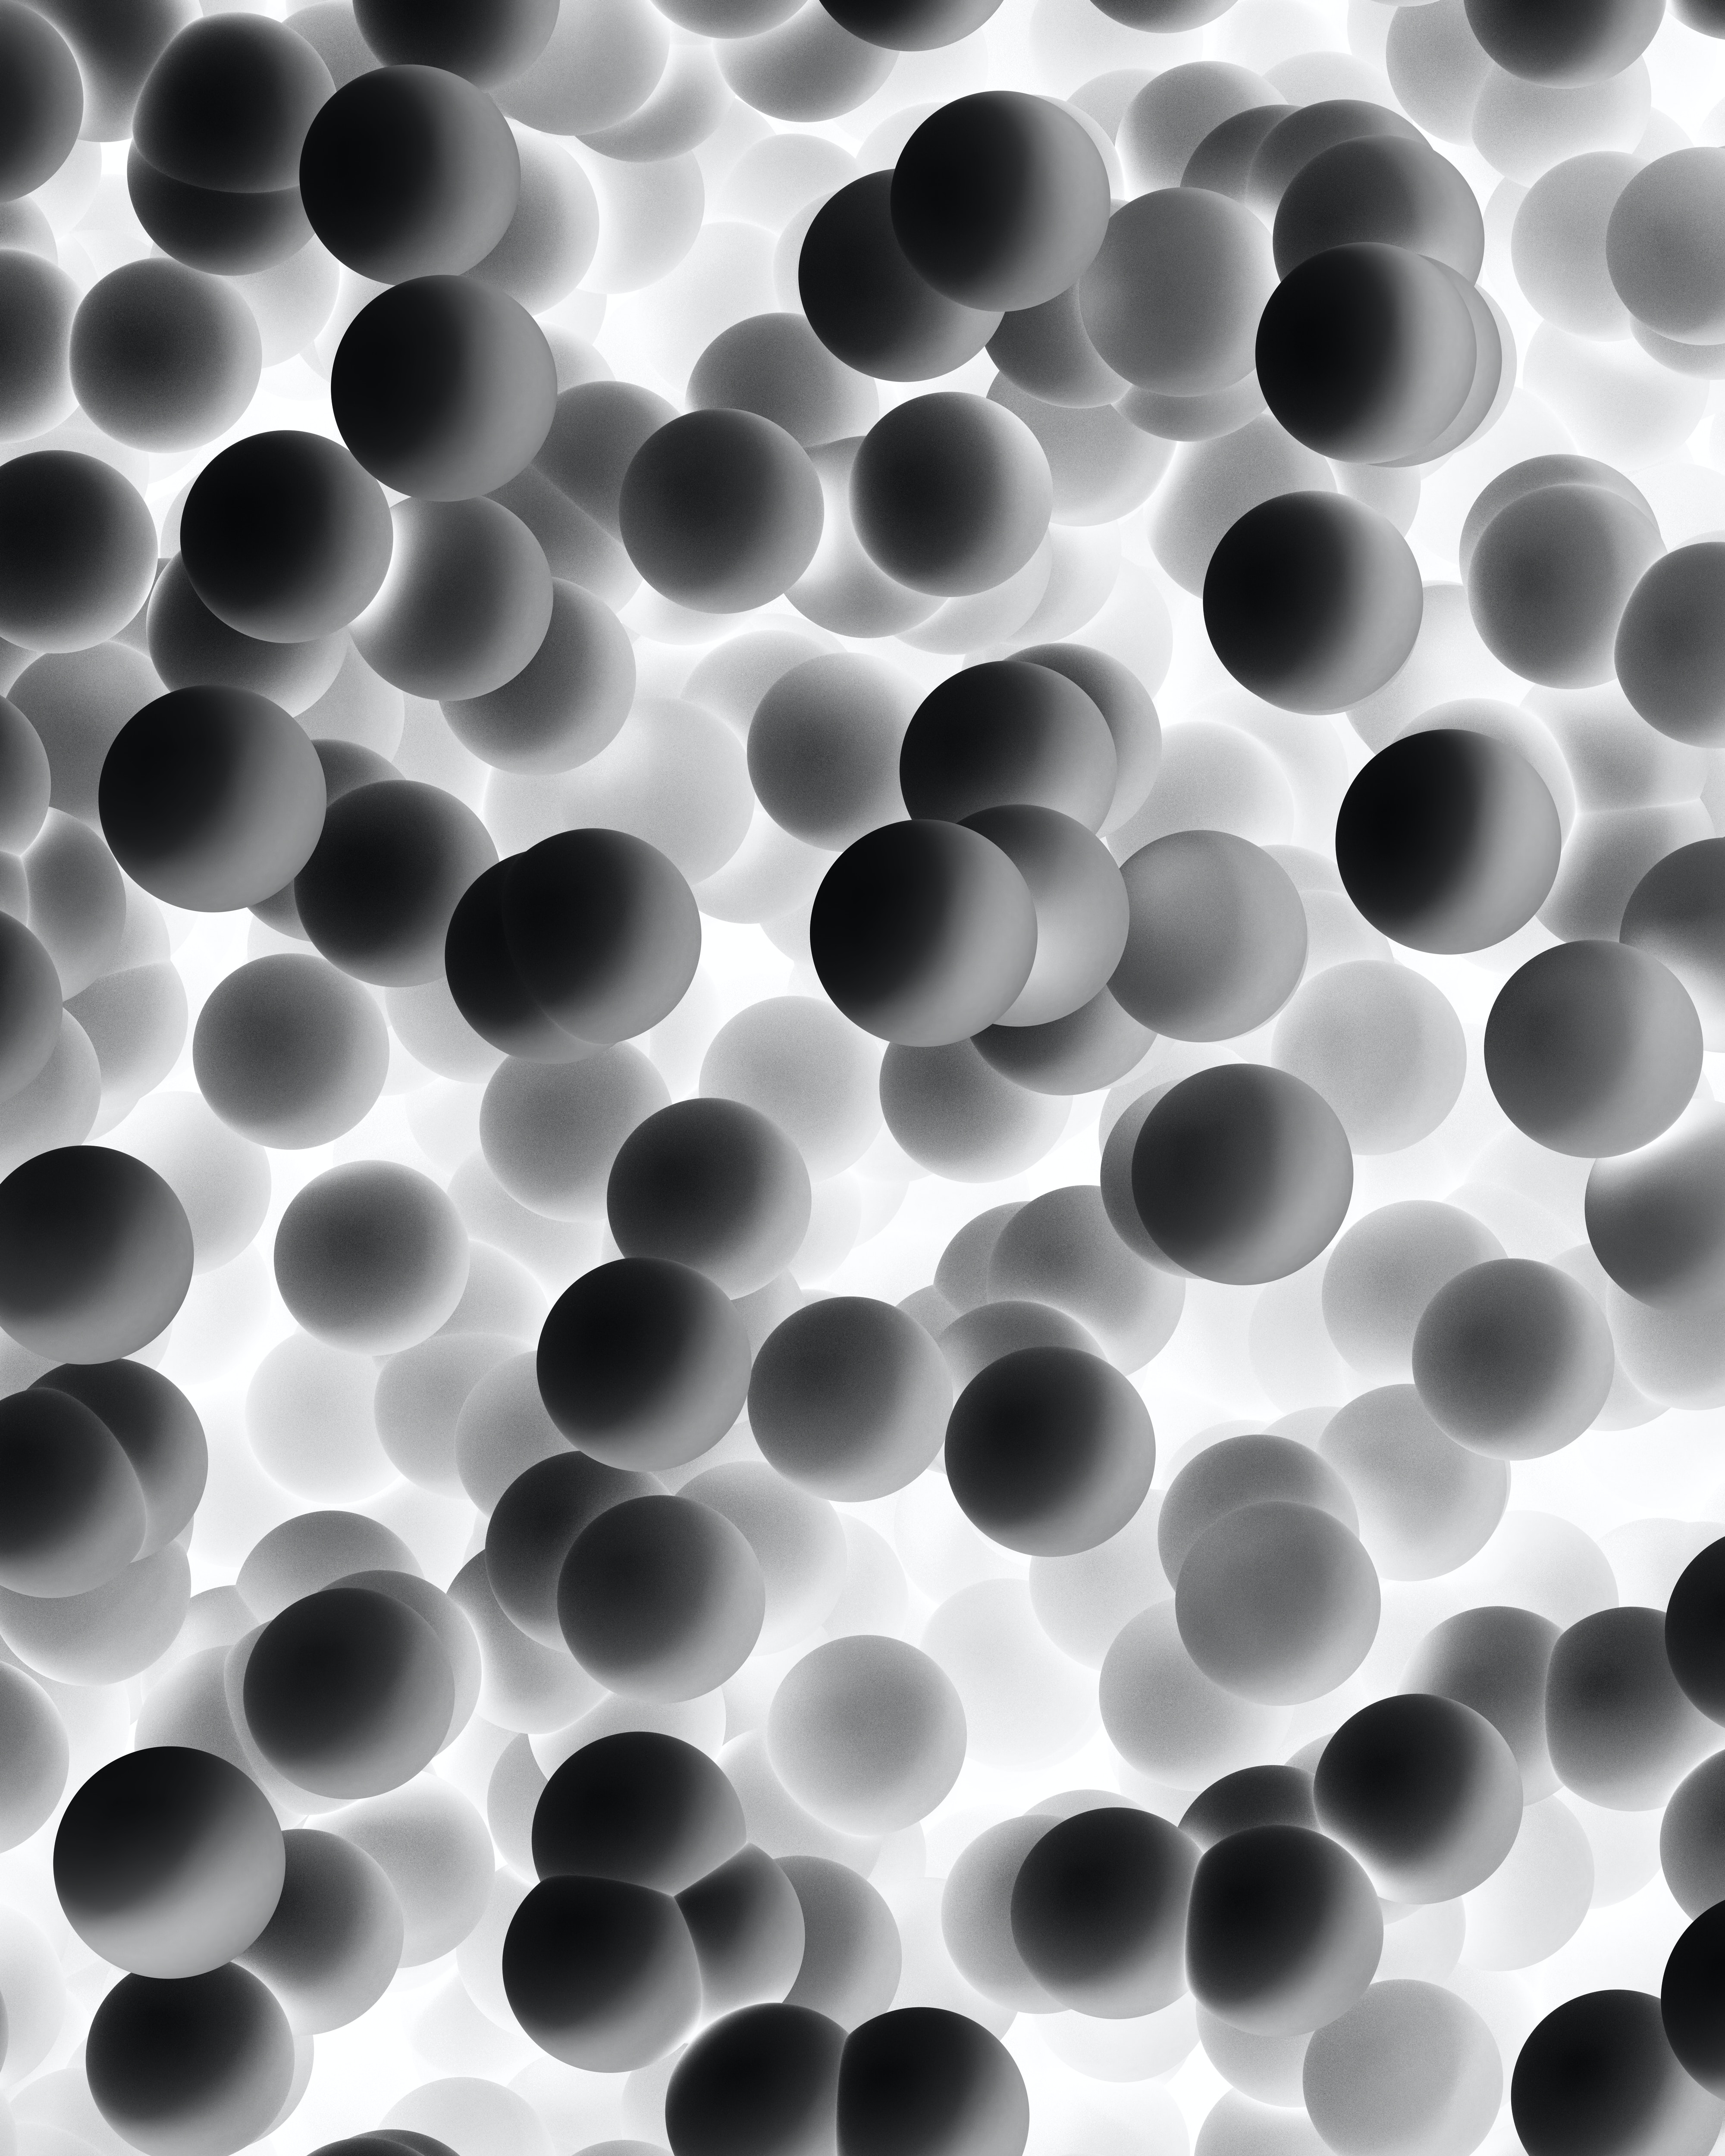
\includegraphics[width=\paperwidth,height=\paperheight]{cover.jpg}%
  }%
}
\hspace{0cm}
\vfill
\, \\\larger[20]\textsf{\textbf{SIOLI'S LECTURES \\ON THERMODYNAMICS}}
\\\smaller[2]MAXIMILIANO SIOLI
\\a.a. 2022-2023
\\~\\ \larger[20]\,\,
\\~\\ \,\,

\vfill
\hspace{0cm}
\end{titlepage}
\makeatother

\tableofcontents
\newpage

\chapter{Introduzione all'approccio termodinamico}
La \textbf{termodinamica classica} si occupa degli \textbf{scambi energetici} tra un \textbf{sistema fisico} e \textbf{l'ambiente circostante}. 
\begin{description}
\item[Sistema] porzione di spazio e/o di materia limitata.
\item[Ambiente] tutto ciò che è esterno al sistema ma può influenzarne il comportamento
\end{description}
Completa e generalizza la trattazione della meccanica classica a qualunque tipo di sistema o fenomeno fisico. \'E caratterizzata da:
\begin{description}
\item[Generalità]
\item[Immortalità] le sue leggi sono rimaste pressoché immutate nel progresso storico della scienza moderna (è valida infatti anche in ambito quantistico!). Si veda la citazione di Einstein:
\begin{quote}
Una teoria è tanto più convincente quanto più semplici sono le sue premesse, quanto più varie sono le cose che essa collega, quanto più esteso è il suo campo di applicazione. Per questo la termodinamica classica mi fece un'impressione così profonda. È la sola teoria fisica di contenuto universale che sono certo non sarà mai sovvertita, entro i limiti in cui i suoi concetti fondamentali sono applicabili (dedicato alla speciale attenzione di quelli che 
sono scettici per principio).
\end{quote}
\end{description}
Nasce dalla necessità dello studio di modalità di conversione del calore in lavoro (e quindi energia meccanica).
\\Lo studio della relazione tra sistema e ambiente (ovvero altri sistemi) si traduce nella descrizione quantitativa del comportamento del sistema e delle sue interazioni. Esistono due approcci: uno macroscopico, proprio della termodinamica \textit{classica}, che prescinde dalla descrizione dei costituenti elementari, e uno microscopico.

\subsection{Approccio microscopico}
Per un sistema di $N$ punti materiali, si definisce il \textbf{microstato (o stato microscopico)} secondo:
\begin{description}
\item[Microstato] insieme di quantità vettoriali che definiscono la descrizione dinamica di tutti i costituenti elementari (le particelle).
\end{description}
Si rappresenta come
\[\{\vec{x}_i, \vec{p}_i\}_{i = 1, ..., N}\]
Con i vettori posizione e i momenti. Ogni quantità vettoriale corrisponde, nello spazio tridimensionale, a tre scalari. Dunque in totale il microstato è un insieme di 6N quantità $\displaystyle \in \, \mathbb{R}$.
\\Noto lo stato del sistema ad un dato istante nel tempo e il campo di forze cui è sottoposto, è possibile studiarne l'evoluzione dinamica nel tempo, impostando un sistema di 3N equazioni differenziali del II ordine scalari (applicando Newton). Si nota che poiché nella II Legge della dinamica compare la derivata seconda della posizione, le leggi della dinamica classica sono \textbf{invarianti per inversione temporale}: si può studiare l'evoluzione sia nel futuro che nel passato.
\[\begin{cases}
m_1 \ddot{ \vec{x}}_1 = \vec{f}_1 = \vec{f}_1^{(e)} + \sum\limits_{i=2}^N \vec{f}_{1i}\\
\quad \vdots\\
m_N \ddot{ \vec{x}}_N = \vec{f}_N = \vec{f}_N^{(e)} + \sum\limits_{i=1}^{N-1} \vec{f}_{Ni}
\end{cases}\]
considerando forze interne ed esterne. La risoluzione richiede $2 \cdot 3N = 6N$ condizioni al contorno scalari, e conduce all'equazione oraria del moto delle particelle.
\\Essa può essere rappresentata come una curva nello \textbf{Spazio delle fasi (o degli stati)}
\begin{description}
\item[Spazio delle fasi] Spazio matematico astratto $6N$-dimensionale i cui punti rappresentano ogni possibile microstato del sistema.
\end{description}
Esiste un vincolo sulla grandezza di $N$? In linea di principio, secondo il determinismo assoluto (classico) incarnato dal \textbf{Demone di Laplace} il problema del moto è sempre risolvibile per qualsiasi numero di particelle: un'intelligenza in grado di conoscere perfettamente lo stato ed il campo di forze può anche conoscere esattamente lo sviluppo passato e futuro.
\\In pratica, tuttavia, $N \tilde N_A = 6 \cdot 10^{23}$ per sistemi normalmente studiati e $N \tilde 10^{80}$ per l'universo osservabile: risulta di fatto impossibile, anche solo con metodi numerici che consentano un margine d'errore accettabile, risolvere il sistema di differenziali.
\paragraph{Crisi del determinismo laplaciano} nel '900 il determinismo classico è stato poi minato da 
\begin{description}
\item[Teoria del caos] una minima (ma inevitabile) incertezza sperimentale di misura sulle condizioni al contorno tende a propagarsi, generando un cono di incertezza con crescita esponenziale, tramite dispersione e amplificazione. Dopo un certo tempo si ha una perdita di informazione sul microstato tanto importante da rendere inutili le previsioni
\item[Principio di indeterminazione di Heisenberg] la descrizione meccanica delle singole particelle è probabilistica: è impossibile conoscere con eguale precisione posizione e momento secondo
\[\Delta x \Delta p \geq \hbar\]
\end{description}
\paragraph{La Dinamica dei sistemi} rappresenta un possibile approccio risolutivo: con le equazioni cardinali si sacrifica la conoscenza esatta del microstato per inglobare l'informazione in pochi parametri rappresentativi dell'intero sistema
\[\begin{cases}
\sum \vec{f_i}^{(e)} = \dot{ \vec{P}} = M \dot{ \vec{v}}_{CM}\\
\sum \vec{\mathcal{M}_i}^{(e)} = \dot{ \vec{L}}_\Omega = \dv[•]{•}{t} \big(\vec{L}_{CM} + \vec{r}_{CM} \times \vec{P}\big)\\
\end{cases}\]
Per $N < 3$ il sistema impostato è risolvibile analiticamente (le due equazioni cardinali vettoriali, e quindi corrispondenti 6 scalari, del I ordine sono sufficienti fino a $3N = 6$, ovvero $N=2$ d.o.f.): per ordini di grandezza maggiori è necessaria l'imposizione di vincoli che contengano il numero di gradi di libertà. Si ha il corpo rigido
\begin{description}
\item[Corpo rigido] un sistema di punti materiali le cui distanze reciproche sono fisse.
\end{description}
Si noti che esso è un costrutto puramente matematico, non esiste nella realtà (l'azione istantanea a distanza per mantenere la perfetta rigidità viola la località relativistica). Il numero dei suoi gradi di libertà è mantenuto costante a $6$, corrispondenti a
\begin{description}
\item 3 per la posizione del centro di massa +
\item 3 per gli angoli di Eulero. Questi descrivono l'orientazione relativa di una terna ortogonale propria del corpo, definita fissando 3 punti ed il CM, rispetto a una terna fissa in un SdR inerziale.
\end{description}
Un altro possibile approccio è quello di uno dei due rami della trattazione termodinamica.
\paragraph{La termodinamica statistica} si basa sulla conoscenza di opportuni valori medi di grandezze microscopiche reinterpretabili in termini macroscopici, ovvero in termini di fenomeni e proprietà emergenti. Poiché le forze in gioco nella trattazione sono tendenzialmente la gravità e l'elettromagnetismo, essa è applicabile fino a energie $\tilde 10^{9} \, \mathrm{eV}$. 
\\Essa è efficace sotto l'assunto di fluttuazioni contenute. Ipotizzando un regime poissoniano per l'incertezza, si ha
\[\frac{\delta N}{N} = \frac{1}{\sqrt{N}} \xrightarrow[N \rightarrow +\infty]{} 0\]
dunque la trattazione è valida per $N$ elevati. In genere il limite del campo di applicabilità dipende dal modello specifico.

\section{Approccio macroscopico: la termodinamica classica}
La termodinamica classica descrive un \textbf{sistema termodinamico} tramite il suo \textbf{macrostato}, caratterizzato da \textbf{coordinate termodinamiche macroscopiche} (pressione, volume, densità, composizione chimica, etc.) indipendenti dal tempo.
\begin{description}
\item[Sistema termodinamico] un sistema fisico descrivibile attraverso coordinate termodinamiche.
\end{description}
Le c.t. possono essere
\begin{description}
\item[Estensive] ovvero avere proprietà di \textbf{additività} (variano con la quantità di materia nel sistema)
\item[Intensive] ovvero \textbf{non} essere additive
\end{description}
Tra i due tipi vi sono relazioni peculiari: si possono infatti determinare \textbf{coppie di variabili coniugate} $(int, \, est)$
\paragraph{Il prototipo di sistema studiato nel corso} è un \textbf{sistema idrostatico} costituito da un gas in un cilindro con un pistone.
\begin{description}
\item[Sistema idrostatico] sistema termodinamico che esercita una pressione uniforme nei confronti dell'ambiente
\end{description}
All'equilibrio esso è un esempio di \textbf{sistema semplice}.
\begin{description}
\item[Sistema semplice] un sistema termodinamico completamente descrivibile a livello macroscopico tramite 3 c.t., di cui due indipendenti. Definito 'sistema XYZ' da Zemansky.
\end{description}
\subsection{Equilibrio termodinamico}
Si definisce secondo
\begin{description}
\item[Equilibrio termodinamico] stato di un sistema termodinamico tale per cui le coordinate termodinamiche rimangono immutate nel tempo (a meno di fluttuazioni statistiche)
\end{description}
Si osserva che fuori dall'equilibrio in realtà le c.t. non hanno valori uniformi all'interno del sistema (vi sono forti disomogeneità): esse infatti caratterizzano un sistema \textbf{solo all'equilibrio!}
\\L'oggetto di studio del corso è infatti la \textit{termodinamica assiomatica dei sistemi all'equilibrio} (vecchio nome), in quanto oltre a quanto detto si basa su assiomi di derivazione sperimentale. La termodinamica classica è quindi in qualche modo una 'termostatica'.
\paragraph{Si ha l'equilibrio termodinamico} quando sono verificati contemporaneamente:
\begin{description}
\item[Equilibrio meccanico] ovvero uno stato in cui non si hanno parti meccaniche in moto (considerando il sistema nel complesso, a livello macroscopico)
\item[Equilibrio chimico] ovvero le concentrazioni e la composizione non variano nel tempo
\item[Eq. termico] ovvero la temperatura del sistema si mantiene costante
\end{description}

Si definiscono quindi
\begin{description}
\item[Universo termodinamico] l'insieme del sistema e dell'ambiente circostante
\[U = S + A\]
\end{description}
\begin{center}

\begin{tabular}{c|c c}
& \multicolumn{2}{c}{Scambia}\\
& Materia & Energia\\\hline
Aperto & sì & sì\\
Chiuso & no & sì\\
Isolato & no & no

\end{tabular}

\end{center}
Si nota che la definizione del confine tra $S$ e $A$ per casi specifici presenta un qualche grado di arbitrarietà e può variare a seconda delle esigenze della trattazione.

\subsection{Gradi di libertà termodinamici}
Non tutte le c.t. sono necessarie per caratterizzare completamente lo stato di un sistema termodinamico all'equilibrio: sono sufficienti quelle indipendenti.
\begin{description}
\item[Grandezze indipendenti] possono assumere valori arbitrari
\item[Grandezze dipendenti] date due gr. $x$, $y$ indipendenti, una terza $z$ è dipendente se $\exists f'(x,y) = z$ o, alternativamente
\[\exists \, f \, : \, f(x,y,z) = 0\]
ovvero è possibile definire un'equazione di stato
\item[Equazione di stato] funzione delle c.t. di un sistema che ha valore costante ($0$) e dunque esprime un vincolo tra valori di queste.
\item[Gradi di libertà termodinamici] numero di c.t. \textbf{intensive} indipendenti di un sistema
\end{description}
Il numero di d.o.f. termodinamici è dato dalla 
\begin{center}

\framebox{
\parbox{\linewidth}{
\vspace{0.3cm}
\textbf{REGOLA DELLE FASI DI GIBBS} \hfill $\displaystyle \nu = C + 2 - F$
\vspace{0.3cm}
}
}
\end{center}
ove $C$ sono le componenti e $F$ le fasi.
\begin{description}
\item[Fase] regione di spazio (o di un sistema termodinamico) con proprietà uniformi della materia. Corrispondono agli stati di aggregazione di una sostanza.
\end{description}
$\nu$ può variare con l'energia (ovvero con la temperatura), in quanto a seconda del superamento di date soglie possono manifestarsi, oltre alla fase solida, in ordine: la fase liquida, quella aeriforme (le uniche altre trattate nel corso), il plasma, il QGP, plasma di quark e gluoni. Le leggi della termodinamica classica sono universalmente applicabili a tutti gli stati di aggregazione (!).

\chapter{Principio Zero e Temperatura}
Si dimostra come il concetto di temperatura emerga spontaneamente da quello di equilibrio termico, tramite il \textbf{Principio Zero della Termodinamica}.
\\Siano dati due sistemi semplici $A$, $B$ con c.t. indipendenti $(x,y)$ e $(x',y')$ rispettivamente. Siano essi posti a contatto attraverso una \textbf{parete}.
\begin{description}
\item[Parete] superficie (reale o figurata) che delimita il sistema nello spazio metrico completo
\end{description}
Si definiscano quindi due tipi di pareti:
\begin{description}
\item[Adiabatica] se mantiene inalterate le coppie di c.t. dei due sistemi che la determinano
\item[Conduttrice (o diatermica)] se $\displaystyle \exists \, f(x,y; x', y') = 0$	 \\ovvero le coppie di c.t. si modificano in modo non indipendente
\end{description}
Si enuncia una prima definizione di equilibrio termico
\begin{quote}
Due sistemi a contatto attraverso una parete conduttrice sono all'equilibrio termico.
\\Equivalentemente, due sistemi si dicono all'equilibrio termico se sono in stati tali per cui se posti a contatto tramite una parete diatermica si avrebbe un sistema complessivo in equilibrio termico.
\end{quote}
Siano $A$, $B$ separati da parete adiabatica ma a contatto termico con un medesimo terzo sistema $C$, descritto da $(x'', y'')$. Si osserva un fondamentale fatto sperimentale, elevato al rango di principio:
\begin{center}

\framebox{
\parbox{\linewidth}{
\vspace{0.3cm}
\textbf{PRINCIPIO ZERO} due sistemi in equilibrio termico con un terzo sono in equilibrio termico fra loro.
\vspace{0.3cm}
}
}

\end{center}
Ovvero $A$ e $B$ sono in equilibrio termico fra loro. Si dimostra ora la derivazione del concetto di temperatura:
\begin{proof}
Per quanto visto, le ipotesi comportano
\[\exists \, f(x,y; x'', y'') = 0 \quad \exists \, f(x', y'; x'', y'') = 0\]
supponendo sia possibile isolare una variabile in funzione delle altre (ovvero sia soddisfatto il Teorema di Dini) si ha
\[\displaystyle \begin{cases} y'' = g_{AC} (x,y; x'') \\ y'' = g_{BC} (x', y'; x'') \end{cases} \implies g_{AC} (x,y; x'') = g_{BC} (x', y'; x'')\]
Invocando ora il Principio Zero, $\displaystyle \exists \, f_{AB}(x,y;x',y') = 0$ in 	quanto all'eq. fra loro. Tale equazione dev'essere riconducibile a quella ottenuta sopra, in quanto descrivono il medesimo sistema. Ciò implica inoltre che la dipendenza da $x''$ dev'essere la medesima, in modo da essere fattorizzabile. Sia quindi
\[\begin{cases} g_{AC} (x, y; x'') = h_A (x,y) \cdot \psi_C (x'') \\ g_{BC} (x', y'; x'') = h_B(x',y') \cdot \psi_C (x'') \end{cases} \implies h_A(x,y) = h_B(x',y')\]
Applicando analogamente ad $A$ e $C$ all'equilibrio con $B$ si ottiene
\[h_A(x,y) = h_B(x',y') = h_C (x'', y'')\]
Ovvero \textit{esiste una funzione delle coordinate termodinamiche indipendenti che assume il medesimo valore in sistemi all'equilibrio termico fra loro}.
\\Si definisce dunque la \textbf{temperatura empirica} $\displaystyle \equiv h = h_A(x,y) = h_B(x',y') = h_C (x'', y'')$ (il suo valore corrisponde al \text{valore} assunto dalla funzione $h_i$ di ogni sistema all'eq., mentre non necessariamente le espressioni analitiche sono uguali!)	
\end{proof}
Ponendo $h_A(x,y) = t$ costante e analogamente per $B$ si ottengono una curva nel piano $x-y$ e una nel piano $x'-y'$ tali per cui qualsiasi coppia di un punto della prima e uno della seconda descrive stati di $A$ e $B$ all'equilibrio termico fra loro. Si definisce
\begin{description}
\item[Isoterma] Fissato lo stato di un sistema, \textbf{l'isoterma di un altro sistema} è il luogo dei punti nello spazio delle n-ple di coordinate indipendenti corrispondenti a stati in equilibrio termico con tale stato fissato
\end{description}
Le curve ottenute sono dette anche \textbf{isoterme corrispondenti}.
\section{Termometria}
Il Principio Zero permette la realizzazione del \textbf{termoscopio}, che permette di determinare se un sistema è all'equilibrio termico (ha la stessa temperatura empirica) con lo strumento. Per costruire una scala è necessario associare in modo univoco l'isoterma di appartenenza (ovvero il valore di $t$) ad un dato stato $(x,y)$. Si deve dunque costruire una curva che intercetti le isoterme nel piano $x-y$. 
\\Il procedimento più semplice consiste nel fissare (congelare) una variabile, ad esempio $y$, ed utilizzare $x$ come \textbf{variabile termometrica}. Si definisce quindi una \textbf{funzione termometrica} $\theta(x)$: la scelta più semplice è quella di una funzione lineare $\theta(x) = ax + b$. La determinazione dei parametri corrisponde quindi alla \textbf{taratura} della scala.
\\Per 2 parametri sono necessari altrettanti punti fissi, il che implica la necessità di determinare due sistemi facilmente riproducibili cui assegnare valori arbitrari di $t$:
\[\begin{cases} \theta (x_1) = a x_1 + b \\ \theta (x_2) = a x_2 + b

\end{cases} \implies \begin{cases} a = \frac{\theta (x_1) - \theta (x_2)}{x_1 - x_2} \\ b = \frac{\theta (x_2) x_1 - \theta (x_1) x_2}{x_1 - x_2}

\end{cases}\]

\paragraph{Scala Celsius} si pone
\begin{itemize}
\item $\theta_1 = 100$ con $S_1 \equiv$ acqua bollente a $p_{atm}$
\item $\theta_2 = 0$ con $S_2 \equiv$ acqua che congela a $p_{atm}$
\end{itemize}
da cui si ottiene $\displaystyle \theta(x) = 100 \frac{x - x_0}{x_100 - x_0} °C$ (ad esempio $x = V$)
\\Tale scala, prima della ridefinizione (vd dopo), era nota anche come s. centigrada.

\paragraph{Problemi dell'approccio con interpolazione di due punti} sono 
\begin{itemize}
\item la necessità di uno strumento di misura che abbia capacità termica (vd. dopo) molto minore del sistema in esame
\item La difficoltà do riprodurre con assoluta precisione i sistemi presi a riferimento a scala minima, a causa della sensibilità alla minima variazione di pressione.
\end{itemize}
Per risolvere il secondo problema si utilizza alternativamente una scala con un solo punto fisso: il punto triplo dell'acqua.
\begin{description}
\item[Punto triplo] particolare stato di una sostanza in cui è contemporaneamente presente in fase solida, liquida e aeriforme
\end{description}
La minima variazione di pressione, infatti, impedisce la formazione o il mantenimento dello stato di punto triplo (che è appunto un punto nel diagramma di fase, ovvero richiede una specifica combinazione di valori delle c.t.).
\subsection{Cella di punto triplo dell'acqua}

\subsection{Scala Kelvin}
Si ha quindi la scala $\displaystyle \theta(x) = \frac{\theta(x_3)}{x_3} x$. Si osserva che $\theta_{\mathrm{{}^\circ C}} (x_3) = 0.01 \, \mathrm{{}^\circ C}$ e che l'intercetta all'origine della $\displaystyle \theta_{\mathrm{{}^\circ C}}$ è $\displaystyle -273.15 \, \mathrm{{}^\circ C}$. Dunque fissata $ \theta(x_3) = 273.16$ si ottiene una scala con gradi di medesima ampiezza di quelli Celsius, ovvero medesimo coefficiente angolare. Tale scala è la scala Kelvin:
\[\theta_{\mathrm{K}} (x) = 273.16\frac{x}{x_3} \, \mathrm{K}\]
La conversione è dunque $\displaystyle \theta_{\mathrm{{}^\circ C}} = \theta_{\mathrm{K}} - 273.15$
\\Dopo il 1954 la scala Celsius è stata ridefinita (ottenendo la scala C. propriamente detta) ponendo come punti fissi $(0, -273.15)$ e $(x_3, 0.01)$, di modo da fissare la conversione per semplice offset con la Kelvin.

\subsection{Relazione temperatura - c.t. e sostanza}
La funzione termometrica \textbf{non è} indipendente dalla variabile e dalla sostanza scelta; la relazione è stata infatti imposta e non necessariamente è verificata per ogni sostanza. Si considera ad esempio il caso del volume

\subsubsection*{Digressione matematica} 
Sia dato un sistema descritto da 3 c.t. $V, p, \theta$. $\theta$ dipende dal volume, dunque non è indipendente: esiste una funzione di stato $f (p,V,\theta) = 0$. Si espliciti $V = V(p, \theta)$ e, per studiare il comportamento per variazioni infinitesime, si differenzi (avendolo in tal modo ridefinito come funzione di stato, il volume ammette differenziale esatto). Si ottiene la forma differenziale
\[\dd[•]{V} = \bigg(\frac{\partial V}{\partial \theta}\bigg)_p \dd[•]{\theta} + \bigg(\frac{\partial V}{\partial p}\bigg)_\theta \dd[•]{p}\]
In termini fisici il differenziale è da intendersi come una variazione di volume:
\begin{enumerate}
\item Sufficientemente ridotta rispetto a $V$
\item Sufficientemente grande per contenere un numero statisticamente elevato di costituenti elementari, e dunque non risentire in modo significativo di fluttuazioni
\end{enumerate}
Il procedimento che si sta seguendo è denominato \textbf{passaggio al continuo}.
\paragraph{Il coefficiente di dilatazione volumetrico} $\displaystyle \alpha \equiv \frac{1}{V} \bigg(\frac{\partial V}{\partial \theta}\bigg)_p$ caratterizza l'inerzia termica di un corpo. Per corpi con dilatazione lungo due direzioni trascurabile, o in genere considerando esclusivamente una direzione, si ha il coeff. di dilatazione lineare $\displaystyle \alpha_L \equiv \frac{1}{L}\bigg(\frac{\partial L}{\partial \theta}\bigg)_p$
\\Si dimostra ora che $\alpha \approx 3 \alpha_L$ per piccole variazioni di temperatura
\begin{proof}
Linearizzando in intorno infinitesimo $\displaystyle \bigg(\frac{\partial V}{\partial \theta}\bigg)_p \approx \frac{\Delta V}{\Delta \theta}$, dunque $\alpha \approx \frac{1}{V} \frac{\Delta V}{\Delta \theta}$. Si procede analogamente per $\alpha_L$. Considerando una porzione cubica di volume, si ha $V = L^3$ e $V' = V + \Delta V = (L')^3 = (L + \Delta L)^3$. Dunque $\displaystyle V ( 1 + \alpha \Delta \theta) = L^3 (1 + \alpha_L \Delta \theta)^3$. Si semplifica; per $\Delta \theta \rightarrow 0$ è poi possibile sviluppare il secondo membro in serie di Taylor al primo ordine, ottenendo
\[1 + \alpha \Delta \theta = (1 + \alpha_L \Delta \theta)^3 \approx 1 + 3 \alpha_L \Delta \theta \implies \alpha \approx 3 \alpha_L\]
\end{proof}
\paragraph{Il coefficiente di comprimibilità isoterma} $\displaystyle \frac{1}{k} \equiv - \frac{1}{V} \bigg(\frac{\partial V}{\partial p}\bigg)_\theta$ ove il segno è negativo in quanto aumentando la pressione a temperatura costante si ha una diminuzione del volume.
\\Si nota inoltre che i coefficienti non sono costanti e indipendenti dalle c.t. Infatti $\alpha = \alpha(\theta)$ e $k = k(p)$.
\subsubsection*{Dilatazione termica: POV microscopico}
In presenza di molecole asimmetriche si ha la formazione di dipoli, che danno luogo a forze intermolecolari (presenti anche più debolmente in molecole apolari, ove si hanno Forze di London). Un modello che descrive il potenziale d'interazione intermolecolare è quello di Lennard-Jones:
\[U(r) = \varepsilon \bigg[\bigg(\frac{r_{min}}{r}\bigg)^{12} - 2 \bigg(\frac{r_{min}}{r}\bigg)^6\bigg]\]
ove $r$ è la distanza tra le molecole. La forza (corrispondente alle ff. di Van der Waals) è data secondo $\displaystyle F = - \dv[•]{U}{r}$ (opposto del gradiente): essa è dunque repulsiva a distanze inferiori a $r_{min}$ e attrattiva per superiori.
\\Nel grafico si nota la presenza di un punto di equilibrio in $r_{min}$, in fondo alla \textit{buca di potenziale}. Intercettando orizzontalmente con il valore dell'energia meccanica delle particelle, dall'equazione della conservazione dell'energia $E = U + K = cost$ si determina l'andamento dell'energia cinetica e le caratteristiche del moto molecolare. Per $E < 0$ il grafico è intercettato in due punti: sono la distanza minima e massima, si ha dunque uno \textbf{stato legato}. Per $E > 0$ le molecole sono invece libere.
\\Si osserva che la curva è asimmetrica: aumentando l'energia meccanica la distanza molecolare media aumenta, tendendo a infinito per $E \rightarrow 0$: dunque aumentando l'energia cinetica, che si vedrà essere in valor medio proporzionale alla temperatura, si ha aumento della distanza media tra le molecole, e quindi del volume occupato a pressione costante.

\subsection{Termometro a GP}
\paragraph{Procedura operativa}
\begin{enumerate}
\item Taratura in cella di punto triplo (immersione) $\rightarrow$ determinazione $p_3$
\item Misura secondo $\displaystyle \theta(p) = 273.16 \frac{p}{p_3}$
\end{enumerate}
Si osserva che variando il numero di moli si hanno valori differenti di pressione in corrispondenza del punto triplo. Graficando l'andamento per le varie sostanze si osserva che la relazione $\theta\big(p_3(n)\big)$ è lineare con coefficienti angolari differenti. Tuttavia, per $p_3 \rightarrow 0$ tutte le rette convergono a $\theta = 373.15$.
\\Rimuovendo progressivamente il gas dal bulbo, e dunque aumentandone la rarefazione (ovvero la distanza intermolecolare) si va a 'spegnere' il potenziale di LJ (specifico delle varie sostanze), lasciando come unico contributo energetico l'energia cinetica, che si può già evincere corrisponda alla temperatura: dunque \textbf{tutti i gas hanno il medesimo comportamento nel limite} $p 	\rightarrow 0$, ovvero a volume costante $r \rightarrow \infty$.
\subsubsection*{Il Gas Perfetto}
\'E quindi possibile definire un modello fisico (approssimazione teorica ma estremamente efficace) denominato \textbf{Gas Perfetto}, che descrive il comportamento di qualunque gas nel limite di elevata rarefazione (unica condizione necessaria!), permettendo la definizione e l'utilizzo della $\theta$ misurata con il termometro a gas. 
\\Il limite fisico di utilizzo di tale strumento è dato dalla più bassa temperatura di liquefazione di un gas, ovvero i $0.5 \, \mathrm{K}$ dell' $\mathrm{{}^3He}$. Per coprire l'intervallo $[0, 0.5[$ sarà necessario svincolare completamente il concetto di temperatura dalla sostanza termometrica.

\subsection{Scala internazionale delle Temperature (ITS)}
\'E definita una scala con una serie di punti fissi misurati con grande precisione tramite termometri a GP. Per misure di valori intermedi essi sono poi utilizzati per tarare altri tipi di termometri (pirometri, ovvero misuratori di radiazione emessa, t. a resistenza di platino, termocoppie platino-rodio o PRT e altri). Essa non sostituisce le scale di riferimento ma ha uno scopo pratico. Definita la prima volta come IPTS (P = Practical) nel 1968, secondo lo standard ITS 90 ha come estremi il punto triplo dell'Idrogeno a $13.8 \, \mathrm{K}$ e il punto di solidificazione del Rame a $1357.77 \, \mathrm{K}$.

\chapter{Sistemi Termodinamici}
Una lunga serie di esperienze ha permesso di determinare le relazioni tra le c.t. dei gas nel limite di GP, fino all'ottenimento dell'\textit{equazione di stato dei gas perfetti}.
\begin{center}
\framebox{
\parbox{\linewidth}{
\vspace{0.3cm}
\textbf{LEGGI DEI GAS PERFETTI}
\begin{description}
\item[I Legge di Gay-Lussac] \hfill a $p$ cost \hspace{2cm} $\displaystyle V = V_0 \beta \theta$ ($V \propto \theta$)
\item[II Legge di Gay-Lussac] \hfill a $V$ cost \hspace{2cm} $\displaystyle p = p_0 \beta \theta$ ($p \propto \theta$)
\item[Legge di Boyle] \hfill a $n, \theta$ cost \hspace{2cm} $\displaystyle V = \frac{cost}{p}$ ($\displaystyle V \propto \frac{1}{p}$)
\item[Legge di Avogadro] \hfill a $p, \theta$ cost \hspace{2cm} $\displaystyle V = cost' \cdot n$ ($V \propto n$)
\item[Equazione di stato dei GP] \hfill $\boxed{\displaystyle pV = nR \theta}$
\end{description}
\vspace{0.3cm}
}
}
\end{center}
Dove i valori con pedice $0$ indicano le c.t. alla temperatura di $0 \celsius$, la temperatura è espressa in $\kelvin{}$ e $R$ è la costante dei gas.
\\Si osserva che consegue dall'equazione che in condizioni normali tutti i gas hanno il medesimo volume molare, corrispondente a $22.4 \, \mathrm{L \, mol^{-1}}$
\\Si ricava inoltre in modo immediato:
\[\alpha = \frac{1}{V} \pdv[•]{•}{\theta} \bigg(\frac{nR \theta}{p}\bigg) = \frac{nR}{pV}= \frac{1}{\theta}\]
\[\frac{1}{k} = - \frac{1}{V} \pdv[•]{•}{p} \bigg(\frac{nR\theta}{p}\bigg) = \frac{nR\theta}{V p^2} = \frac{1}{p}\]

\subsection{Isoterme}
Dall'equazione di stato si ottengono le equazioni delle isoterme nel piano $p-V$, secondo
\[p(V; \theta) = \frac{nR\theta}{V}\]
esse sono dunque delle iperboli. 

\section{Trasformazioni termodinamiche}
\begin{description}
\item[Trasformazione termodinamica] processo in cui variano le proprietà (e dunque le c.t.) di un sistema termodinamico
\end{description}
Tramite trasformazioni cambia lo stato del sistema, ovvero la sua configurazione. Tuttavia, durante la trasformazione è impossibile rappresentare stati intermedi sui grafici: per quanto notato anche in precedenza, non si tratta di stati all'equilibrio, e dunque le c.t. non hanno valori uniformi.
\\Tuttavia è possibile costruire un modello, quello delle \textbf{trasformazioni quasistatiche}.
\begin{description}
\item[Trasformazione quasistatica (q.s.)] una trasf. termodinamica che procede attraverso una successione di infiniti stati all'equilibrio differenti di infinitesimi.
\end{description}
Si hanno quindi curvi corrispondenti a trasformazioni isoterme (le curve già viste), isobare (a pressione costante) e isocore (a volume costante).
\\A livello pratico, tali trasformazioni sarebbero realizzabili secondo le seguenti procedure:
\begin{itemize}
\item \textbf{Isobara} per ogni variazione infinitesima di volume del sistema idrostatico, ottenuta diminuendo il peso posto sul pistone, lo si pone a contatto con un termostato con temperatura maggiore di un infinitesimo del precedente, iterando fino al raggiungimento del volume finale
\item \textbf{Isocora} per ogni variazione infinitesima di temperatura, ottenuta sostituendo il termostato come in precedenza, si incrementa la pressione sul pistone aggiungendo masse infinitesime ulteriori.
\end{itemize}

\section{Gas Reali}
Lontano dal limite di G.P., è necessario apportare delle correzioni all'equazione di stato per tenere conto delle proprietà specifiche dei vari gas. Sono possibili due approcci. 
\subsection{Sviluppo del viriale}
Si definisce il \textbf{fattore di compressione} $\displaystyle z \equiv \frac{pV}{nR\theta}$, che quantifica l'allontanamento dal modello ideale. Quindi si sviluppa in serie in $p$ per $p \rightarrow 0$:
\[z(p) = 1 + Ap + Bp^2 + C p^3 + ...\]
con i coefficienti da determinarsi tramite fit sui dati sperimentali (dipendono dalla temperatura). Alternativamente si sviluppa nel volume molare $\molvol = \frac{V}{n} \propto \frac{1}{\rho}$:
\[z\big(\frac{1}{\molvol}\big) = 1 + \frac{A'}{\molvol} + \frac{B'}{\molvol^2} + ...\]
\subsection{Equazione di Van der Waals}
Alternativamente si adotta un approccio \textit{empirico}, valutando modifiche all'equazione sulla base dello studio dell'andamento del potenziale di L-J. 
\\Per distanze inferiori a $r_{min}$ domina il termine repulsivo $\propto r^{-12}$, fino ad un \textbf{muro di potenziale} per $r \rightarrow 0$: ciò corrisponde all'impenetrabilità (e quindi non compenetrabilità) delle molecole, che non possono essere quindi assunte puntiformi. Esse occupano un volume minimo costante proporzionale al loro numero, e quindi alle moli. Esso è denominato covolume
\[V_{reale} = V_{ideale} + \underbrace{b \cdot n}_{cov.} \]
Si osserva poi che la pressione (come sarà poi visto approfonditamente) è la manifestazione macroscopica degli urti delle molecole sulle pareti che delimitano il sistema idrostatico. La presenza di interazioni intermolecolari attrattive per distanze maggiori a $r_{min}$, ove domina il termine $\propto - r^{-6}$, diminuisce l'impulso scambiato con le pareti, riducendo la quantità di moto delle molecole $^1$; invece un maggior numero di molecole implica un numero maggiore di impatti. Dunque la diminuzione del contributo della singola molecola $\dd[•]{p}$ è proporzionale a $\rho$ per $^1$, mentre la diminuzione complessiva è data da $N \cdot \dd[•]{p}$. Dunque $\displaystyle \dd{p}_{tot} \propto \rho^2$, ovvero $\displaystyle \dd{p}_{tot} \propto \frac{n^2}{V^2} = \frac{1}{\molvol^2}$. Indicando la costante di proporzionalità con $a$ si ha 
\[p_{reale} = p_{ideale} - \underbrace{a \frac{n^2}{V^2}}_{\dd{p}}\]
Sostituendo nell'eq. di stato si ottiene
\begin{center}

\framebox{
\parbox{\linewidth}{
\vspace{0.3cm}
\textbf{EQ. DI STATO DI VAN DER WAALS} \hfill $\displaystyle \bigg(p + a\frac{n^2}{V^2}\bigg) (V - bn) = nR\theta$ \quad \bigg| \quad $\displaystyle \bigg(p + \frac{a}{\molvol^2}\bigg) (\molvol - b) = R \theta$
\vspace{0.3cm}
}
}

\end{center}
ove $a$, $b$ sono dette \textit{costanti di Van der Waals} specifiche di ogni gas. Si osserva che in condizioni standard le correzioni relative sul volume e sulla pressione sono nell'ordine dello $0.1\%$. 
\\Ottenendo l'espressione di $p(V)$ si rappresentano quindi le curve nel piano $p-\molvol$), considerando in particolare le isoterme. 
\[p(V) = \frac{nR\theta}{\molvol - b} - \frac{a}{\molvol^2}\]
\begin{itemize}[label=$\square$]
\item Per $\theta$ elevato il primo termine risulta dominante, dunque per $b$ ridotto la curva tende all'iperbole equilatera dei GP, con asintoto a sinistra a $\molvol = b$ (incomprimibilità!)
\item Per un particolare valore di temperatura, definito $\theta_C$ (critico) si ha un flesso orizzontale. Imponendo l'annullamento della derivata prima e seconda della pressione rispetto al volume si ottiene:
\[\mathrm{v}_C = 3 b \quad \theta_C = \frac{8 a}{27 R b} \quad z_C = \frac{p_C \mathrm{v_C}}{R \theta_C} = \frac{3}{8} = 0.375\]
\begin{proof}
\[\begin{cases} \displaystyle \pdv[•]{p}{\molvol} = 0 \\ \\\displaystyle \pdv[2]{p}{\molvol} = 0
\end{cases} \implies \begin{cases} \displaystyle \frac{2a}{\molvol^3} = \frac{R \theta}{(\molvol - b)^2}\\ \\\displaystyle \frac{2 R \theta}{(\molvol - b)^3} = \frac{6a}{\molvol^4}
\end{cases} \implies \begin{cases} \displaystyle \molvol = 3b \\ \\ \displaystyle 2a(2b)^2 = R \theta (3b)^3
\end{cases} \implies \begin{cases} \displaystyle \theta_C = \frac{2a (4b^2)}{R (27b^3)} = \frac{8a}{27b} \\ \\ \displaystyle \molvol_C = 3b
\end{cases} \implies\]
\[\implies p_C = \frac{R \theta_C}{2b} - \frac{a}{9b} = \frac{a}{27b^2} \implies z_C = \frac{p_C \molvol_C}{R \theta_C} = \frac{3}{8} 0.375\]
Che si osserva essere indipendente dalla sostanza (come verificato sperimentalmente).
Viceversa è anche possibile ricavare le costanti di Van der Waals dalla \textbf{curva critica} secondo:
\[a = \frac{9}{8} R \theta_C \molvol_C \hfill b = \frac{\molvol_C}{3}\]
\end{proof}
\item Per $\theta < \theta_C$ la curva ha un andamento simil-sinuisoidale con massimi e minimi. Tuttavia per determinati intervalli ciò non corrisponde a quanto osservato sperimentalmente: raggiunto un certo valore $V_G$ del volume (o $\molvol_G$ corrispondente) la diminuzione del volume non comporta alcuna variazione della pressione. Si osserva invece la formazione di condensa: si sta infatti verificando una transizione di fase (verso la f. liquida). Una volta completata la transizione, ovvero raggiunto il $V_L$, la curva diviene pressoché verticale, a causa dell'incomprimibilità dei liquidi.
\end{itemize}
Diminuendo ulteriormente la temperatura, si osserva che i valori di $V_L$ e $V_G$ si allontanano. Effettuando un inviluppo sui segmenti orizzontali per le varie temperature subcritiche, ovvero determinando una curva tangente ai punti estremi, si ottiene una parabola con vertice in $\theta_C$, dove è tangente all'isoterma.
\\Ciò permette di realizzare il \textbf{Diagramma di Fase} della sostanza, in cui varie porzioni del piano rappresentano le varie fasi, delimitate dalle curve di saturazione.
\\Per stati nella zona sottesa dalla parabola determinata, il vapore si trova in uno stato definito \textbf{vapore saturo}. Per ogni valore di $V$ (o $\molvol$) compreso tra gli estremi del segmento, e per una data temperatura (o equivalentemente una data pressione) il VS raggiunge l'equilibrio quando il processo di liquefazione di molecole del vapore (a causa degli urti anelastici con la superficie) e quello di evaporazione ('liberazione' per agitazione termica delle molecole superficiali) sono bilanciati. In tal caso il numero di moli di molecole nelle due fasi ($n_L$, $n_G$) resta costante, con il rapporto $\displaystyle \frac{n_L}{n_G} = \frac{\molvol_G - \molvol}{\molvol - \molvol_L}$ con $\molvol_i = V_i \big/ n_i$.
\begin{proof}
\[V_L + V_G = n_L \molvol_L + n_G \molvol_G = n \molvol \quad \frac{n_L}{n_G} = \frac{V_L \big/ \molvol_L}{V_G \big/ \molvol_G}\]
Imponendo $n_L + n_G = n$ (sistema chiuso) si ha
\[n_G \molvol_G + n_L \molvol_G = (n_L + n_G) \molvol \implies n_G(\molvol_G - \molvol) = n_L (\molvol - \molvol_L)\]
\end{proof}
Diminuendo il volume resta costante il numero di molecole che passano da una fase all'altra (pelo del liquido resta il medesimo) in quanto dipende esclusivamente dall'agitazione termica, ovvero dalla temperatura. Tuttavia anche la densità si mantiene costante, a spese di $n_G$.
\\~\\Per temperature supercritiche l'energia cinetica delle molecole è troppo elevata perché possa avvenire l'aggregazione e dunque la transizione di fase. Si osserva inoltre che per sistemi aperti l'evaporazione (non l'ebollizione!) si verifica a qualsiasi temperatura, lungo un tempo determinato dalla probabilità di rottura dei legami ad idrogeno, ovvero alla distribuzione delle energie cinetiche (vd Teoria Cinetica).
\subsubsection*{Costruzione di Maxwell}
\'E possibile determinare i valori di $V_L$ e $V_G$ dalla curva prevista dal modello di Van der Waals per temperature subcritiche, tramite un procedimento analitico. 
\\Il metodo della costruzione di Maxwell prevede di tagliare orizzontalmente la curva, di modo da ottenere due aree sottese (una sopra e una sotto la retta orizzontali) uguali. I volumi estremi intercettati sono quelli cercati.
\\Si osserva che per volumi compresi tra $V_L$ e il minimo locale e tra il massimo locale e $V_G$ la derivata della curva è negativa, ovvero si tratta di stati di equilibrio stabile e quindi realizzabili sperimentalmente; per la porzione intermedia invece la derivata positiva implica si tratti di equilibri instabili, e quindi irrealizzabili.

\subsection{Diagrammi di fase di sostanze pure}
Si tratta di diagrammi tridimensionali nello spazio $\theta, V, p$, in cui le curve di saturazione e transizione generano una superficie denominata \textbf{superficie pVT} ($pV\theta$).
\\Le proiezioni della stessa sul piano (p,V) e (p,$\theta$) danno poi i diagrammi di fase bidimensionali.
\subsubsection{Piano (p,T)}
Sono rappresentate le curve di transizione, descritte dalle equazioni di Clausius-Clapeyron (vd più avanti). Per Temperature e pressioni supercritiche, si ha lo stato di \textbf{fluido supercritico}, che presenta proprietà macroscopiche miste di liquidi (densità) e aeriformi (viscosità). Esso è presente, ad esempio, nei vulcani sottomarini (approssimando un andamento con la profondità $\displaystyle p(h) = \frac{h}{10 \mathrm{m}} \, \mathrm{atm}$ si ha $p(2 \mathrm{km}) = 200 \, \mathrm{atm}$!)
\\Si osserva inoltre che la temperatura di ebollizione varia con la pressione (o viceversa) e che è possibile transire di da liquido ad aeriforme diminuendo la pressione a temperatura costante: si ha il processo di \textbf{cavitazione}.
\paragraph{Si applichi Gibbs} per sistema monocomponente:
\begin{itemize}
\item Nelle regioni piene $F = 1$, dunque $N = 2$: il sistema può trovarsi in qualsiasi punto della regione, in quanto le due c.t. sono indipendenti
\item Lungo le curve $F =2$, dunque $N = 1$: gli stati possibili giacciono sulla specifica curva $p(\theta)$
\item Nel punto triplo $F = 3$, dunque $N = 0$: si realizza solo in condizioni specifiche, da cui la variazione di una qualsiasi c.t. intensiva farebbe allontanare il sistema.
\end{itemize}
Si osservi che è possibile applicare la Regola solo per quanto riguarda la proiezione $(p, \theta)$ in quanto si tratta di variabili intensive.

\chapter{Teoria cinetica dei gas}
\section{Interpretazione microscopica: uno schema}
Il seguente schema concettuale generale descrive il processo scientifico:

\begin{center}
* schema *
\end{center}
La teoria di base della TCG è la meccanica newtoniana. Il modello sviluppato è invece il:
\section{Modello cinetico}
Esso è costituito da $N$ molecole moventi di moto rettilineo uniforme all'interno di una scatola cubica, di cui occupano tutto il volume. Le assunzioni di base del modello sono:
\begin{enumerate}
\item $N$ è sufficientemente grande
\item Il covolume è trascurabile, ovvero le molecole possono essere considerate puntiformi
\item Le interazioni a lungo range sono trascurabili (no L-J) e quelle a corto raggio (urti tra molecole e con le pareti) sono completamente elastiche
\item Si ha il \textbf{caos molecolare}, ovvero  \textbf{omogeneità} (la densità è considerabile uniforme) e \textbf{isotropia} (non vi sono direzioni privilegiate per il moto delle particelle, ovvero il gas è macroscopicamente fermo)
\end{enumerate}
Gli assunti 2. e 3. implicano ci si stia ponendo nel campo di applicabilità del modello di Gas Perfetto.

\paragraph{Aria in condizioni standard soddisfa requisiti?} 
\begin{itemize}
\item Si considera un volumetto $V = 1 \, \mathrm{cm^3}$. Si ha $\displaystyle N = \frac{pV}{R \theta} N_A \approx 10^{19}$ molecole, un numero sufficientemente grande per consentire l'approccio statistico (anche su scala locale!)
\item Il $99 \% $ delle molecole è rappresentato da $N_2$ e $O_2$, che presentano una forma a 'fagiolo' con lunghezza maggiore $d = 1.7 \angstrom$. Approssimando a sfere di raggio $d/2$ si ottiene un covolume $\displaystyle = N \frac{4}{3}\pi \bigg(\displaystyle \frac{d}{2}\bigg)^3 \approx 6 \times 10^{-11} \meters{}{}{3}$ e dunque un rapporto $\displaystyle r \equiv \frac{V_{mol}}{V} \approx 6 \times 10^{-5}$
\item Approssimando la disposizione omogenea con una griglia (un reticolo) con molecole nei vertici si determina il passo:
\[N = \frac{V}{\lambda^3} \implies \lambda = \bigg(\frac{V}{N}\bigg)^{\frac{1}{3}} \approx 34 \angstrom \implies r \equiv \frac{\lambda}{d} \approx 20\]
Poiché $d \tilde r_{min}$, a distanze tanto superiori le interazioni sono trascurabili
\item L'omogeneità è già stata assunta nel punto precedente. Se tutte le molecole hanno approssimativamente uguale massa, la condizione di isotropia $\vec{P} = 0$ si traduce in $\displaystyle \sum_i \vec{v}_i = 0$, ovvero per ogni molecola che si muove in una direzione ve ne è una che si muove sulla medesima ma in verso opposto. 
\end{itemize}

\subsection{Pressione}
Si considerano gli urti elastici su una delle pareti della scatola (l'assunzione di isotropia permette di sceglierne una qualsiasi). Sia essa quella di destra, orientata perpendicolarmente all'asse $x$ e indicata in figura con $S_x$.
\\Per un urto elastico con $M_{parete} \gg m_{mol}$ si ha:
\[\begin{cases} \displaystyle v_{ix}' = - v_{ix} \\ \\ \displaystyle v_{iy}' = v_{iy} \implies \Delta q_{iy} = 0\\ \\ \displaystyle v_{iz}' = v_{iz} \implies \Delta q_{iz} = 0
\end{cases} \implies \Delta q_{ix} = \Delta q_i = - 2m v_{ix}\]
In un dato $\Delta t$, il numero di urti sulla parete della $i$-esima particella dipende dal solo moto su $x$ (in quanto il modulo delle altre componenti rimane invariato e i tre moti sono indipendenti). La variazione totale della quantità di moto su $x$ è quindi calcolata moltiplicando la variazione per ogni particella per il numero di urti corrispondenti e sommando sulle particelle
\[n°_{urti}(i) = \frac{|v_{ix}| \Delta t}{2L} \implies |\Delta Q_x| = \sum\limits_{i=1}^N |\Delta q_{ix}| \cdot n°_{urti}(i) = \sum\limits_{i=1}^N \frac{2 m |v_{ix}| \cdot |v_{ix}| \Delta t}{2L} = \frac{m \Delta t}{L} \sum\limits_{i=1}^N v_{ix}^2\]
assunta la massa uniforme. La forza media è data dalla variazione di quantità di moto complessiva, ovvero l'impulso esercitato, sull'intervallo di tempo. La pressione si ottiene quindi dividendo tale forza per la superficie su cui è applicata:
\[|F_x| = \frac{|\Delta Q_x|}{\Delta t} = \frac{m}{L} \sum\limits_{i=1}^N v_{ix}^2 \implies p_x = \frac{|F_x|}{S_x} = \frac{m}{S_x \cdot L} \sum\limits_{i=1}^N v_{ix}^2 = \frac{m}{V} \sum\limits_{i=1}^N v_{ix}^2\]
Si ricava analogamente l'espressione per pareti ortogonali alle altre due direzioni, ovvero $S_y$ e $S_z$. Per $N$ grande si applica la condizione di isotropia, ovvero si assume che i valori di $v_{ij}$ siano equamente distribuiti sulle tre direzioni $j = x, y, z$. Ciò implica
\[p_x = p_y = p_z \equiv p\]
ovvero si ha pressione idrostatica: si è di fatto ricavato il \textbf{Principio di Pascal}, secondo cui la pressione è una grandezza scalare indipendente dall'orientamento della superficie su cui è applicata. Dunque
\[p = \frac{1}{3}(p_x + p_y + p_z) = \frac{m}{3V} \sum\limits_{i=1}^N [v_{ix}^2 + v_{iy}^2 + v_{iz}^2] = \frac{m}{3V} \sum\limits_{i=1}^N v_{i}^2 \implies
pV = \frac{m}{3}\sum\limits_{i=1}^N v_{i}^2\]
Si introduce quindi la \textbf{velocità quadratica media} $\langle v^2 \rangle$, definita come valore di aspettazione del quadrato del modulo delle velocità molecolari,  e successivamente l'\textbf{energia cinetica molecolare media} $\langle \varepsilon \rangle$:
\[\langle v^2 \rangle \equiv \mathbb{E}[v^2] = \frac{\sum_i v_i^2}{N}\implies pV = \frac{m}{3} N \langle v^2 \rangle = \frac{2}{3} N \bigg(\frac{1}{2}m \langle v^2 \rangle\bigg) = \frac{2}{3}N \big\langle \frac{1}{2}mv^2 \big\rangle = \frac{2}{3}N \langle \varepsilon \rangle\]
in quanto la massa è assunta uniforme. Invocando l'equazione di stato dei gas perfetti:
\[nR\theta = \frac{2}{3}N \langle \varepsilon \rangle \implies \varepsilon = \frac{3}{2}\frac{n}{N} R \theta = \frac{3}{2} \frac{R}{N_a}\theta = \frac{3}{2} k_B \theta\]
Si è così stabilito un \textit{ponte macro-micro} tramite l'introduzione di quantità medie che permettono di considerare una caratterizzazione globale del sistema prescindendo dalla conoscenza esatta del microstato.
\\La temperatura è così caratterizzata come grandezza \textbf{emergente} proporzionale al valor medio delle energie cinetiche molecolari, dunque ad esse collegata per via statistica. Tali d.o.f. interni del sistema, \textit{variabili nascoste} microscopiche, producono una quantità misurabile macroscopicamente.
\\~\\Si ha quindi la giustificazione del comportamento dei gas nel limite del GP: se per il potenziale $U \rightarrow 0$, si ha $E \rightarrow \varepsilon$ con $\langle \varepsilon \rangle \propto \theta$.
\paragraph{Osservazioni}
\begin{itemize}
\item La costante di Boltzmann è misurabile sperimentalmente, ad esempio attraverso l'esperimento di Perrin sul moto browniano
\item Dal 2019 $k_B$ è stata assunta come costante fondamentale senza incertezza per la ridefinizione del$\kelvin{}$ da parte del BIPM. In tal modo la precisione della scala non è più vincolata a quella della riproduzione delle specifiche condizioni di $S_3$, è può anzi in futuro divenire arbitrariamente elevata con la possibilità di ridefinizione dei punti fissi.
\end{itemize}
La costante di Boltzmann rappresenta un vero e proprio fattore di conversione tramite cui la temperatura è ridefinita come una grandezza energetica.
\\Difatti la ridefinizione della scala Kelvin è la seguente:
\begin{quote}
$1 \kelvin{}$ corrisponde alla temperatura di una sostanza che ha $\displaystyle \frac{k_B}{2} \joule{}$ di energia cinetica media per grado di libertà cinetico.
\end{quote}
Per il numero di d.o.f. si fa ricorso al \textbf{Teorema di equipartizione dell'energia} (vd più avanti)
\begin{center}

\framebox{
\parbox{\linewidth}{
\vspace{0.3cm}
\textbf{TEOREMA DI EQUIPARTIZIONE DELL'ENERGIA} A ogni d.o.f. che si presenta in forma di termine quadratico (quadraticamente) nel calcolo dell'energia cinetica corrisponde un termine $\displaystyle \frac{1}{2}k_B \theta$ \vspace{0.3cm}
}
}
\end{center}
Dunque
\[\langle \varepsilon \rangle = \frac{\nu}{2} k_B \theta \implies \theta = \frac{2 \langle \varepsilon \rangle}{k_B \cdot \nu}\]
\textbf{RELATIVIT\'A SPECIALE }\hrulefill
\\Il limite superiore alla velocità determinato dalla SR implica un limite ad $\varepsilon$ e dunque a $\theta$? No, in quanto l'espressione classica per l'energia cinetica non vale fuori dal limite classico! Per velocità prossime a $c$, la differenza di energia necessaria ad imprimere un'ulteriore accelerazione diverge; dunque $\theta \rightarrow \infty$.
\\\hrule

\subsubsection{Legge di Dalton}
Siano dati due (o più) GP occupano insieme un dato volume, e noti il rispettivi numeri di moli e le \textit{pressioni parziali}, ovvero le pressioni esercitate da ognuno occupando interamente il volume in assenza degli altri. Si ha: $\displaystyle p_i = \frac{n_i R \theta_i}{V}$ e  $n = \sum n_i$. Si osserva che $\langle \varepsilon_i \rangle = \frac{3}{2} k \theta_i$ e che per la media complessiva si ha: \[\langle \varepsilon \rangle = \frac{\sum n_i \langle \varepsilon_i \rangle}{\sum n_i} \implies \theta = \frac{2\langle \varepsilon \rangle}{3k} = \frac{2 \sum n_i \langle \varepsilon_i \rangle}{3 k \sum n_i} \implies pV = \big(\sum n_i\big) R \frac{2 \sum n_i \langle \varepsilon_i \rangle}{3 k \big(\sum n_i\big)} = R \sum \frac{2}{3k} n_i \langle \varepsilon_i \rangle =\]
\[= R \sum n_i \theta_i = \sum R n_i \theta_i = \sum p_i V \implies p = \sum p_i\]

\section{Distribuzione delle velocità molecolari (di Maxwell)}
Si intende determinare la PDF della variabile continua $v$, corrispondente al modulo della velocità molecolare
\[\rho \, : \, [0, +\infty [ \, \rightarrow \, [0,1[ \enspace t.c. \enspace P(v < v' < v + \dd{v}) = \rho(v)\dd{v}\]
\\Si assume che il sistema in esame sia all'equilibrio termodinamico, e dunque quello termico ($\theta$ è uniforme e costante) e isolato. Qualsiasi sistema che soddisfi tali assunti tenderà a presentare una configurazione di velocità molecolari descritta dalla Maxwelliana; anche partendo da una distribuzione differente in un certo lasso di tempo urti anelastici condurranno alla distribuzione qui derivata.
\\Per ottenere $\rho$ è in primo luogo necessario determinare le distribuzioni delle singole componenti, $f(v_x)$, $f(v_y)$, $f(v_z)$. Si determina quindi la \textbf{PDF congiunta} definita secondo
\[P(v_x < v_x' < v_x + \dd{v_x}, v_y < v_y' < v_y + \dd{v_y}, v_z < v_z' < v_z + \dd{v_z}) = F(v_x, v_y, v_z) \dd{v_x} \dd{v_y} \dd{v_z}\]
ovvero la funzione che quantifica la probabilità che la terna di velocità di una molecola qualsiasi si trovi nel cubetto infinitesimo dello spazio delle velocità.
\\Nell'ipotesi del caos molecolare, le distribuzioni delle tre componenti sono indipendenti, ovvero l'informazione su ciascuna non influisce su quella delle altre. Segue che $F$ sia data secondo:
\[F(v_x, v_y, v_z) = f(v_x) f(v_y) f(v_z) \enspace ^1\]
Inoltre per l'isotropia (che costituisce un \textbf{fatto fisico}) $F$ non può presentare una dipendenza dal verso e/o dalla direzione di $v$: deve essere funzione del solo modulo, ovvero della distanza del punto $(v_x, v_y, v_z)$ dall'origine dello spazio delle velocità$^2$.
\\Da $^1$ e $^2$ si ottiene:
\[F(v_x^2 + v_y^2 + v_z^2) = f(v_x) f(v_y) f(v_z)\]
L'unica funzione in grado di soddisfare entrambe le formulazioni di $F$ è l'\textbf{esponenziale}. \\Infatti $e^{\sum a_i} = \prod e^{a_i}$. Si assume quindi un'\textbf{ipotesi di lavoro} sulla forma di $f$:
\[f(v_i) = \eta e^{\pm \xi v_i^2} \implies
 F(v_x, v_y, v_z) = \eta^3 e^{\pm \xi (v_x^2 + v_y^2 + v_z^2)} = \eta^3 e^{\pm \xi v^2}\]
\'E quindi necessario determinare i due parametri ed il segno dell'esponente (assunto $xi > 0$). Poiché il sistema ha un'energia finita, quest'ultimo dev'essere negativo, di modo da avere probabilità tendenti a $0$ per moduli delle velocità tendenti a $\infty$: $\displaystyle F \xrightarrow[v \rightarrow +\infty]{} 0$
\\Si impone quindi la normalizzazione, considerando il valore noto per l'integrale errore:
\[\int_{-\infty}^{+\infty}f(v_i)\mathrm{d}v_i = \eta \int_{-\infty}^{+\infty}e^{-\xi v_i^2}\mathrm{d}v_i = \eta \frac{1}{\sqrt{\xi}} \int_{-\infty}^{+\infty} e^{-\xi v_i^2}\sqrt{\xi}\mathrm{d}v_i \implies
t = \sqrt{\xi}v_i \implies \eta \frac{1}{\sqrt{\xi}} \int_{-\infty}^{+\infty}e^{-t^2}\mathrm{d}t =\]
\[= \eta \frac{\sqrt{\pi}}{\sqrt{\xi}} = 1 \implies \eta = \sqrt{\frac{\xi}{\pi}}\]
Si impone ora la relazione determinata in precedenza per l'energia cinetica media e dunque la velocità quadratica media, sotto l'assunzione di massa molecolare uniforme:
\[\langle \varepsilon \rangle = \frac{3}{2} k \theta \implies \langle v^2 \rangle = \frac{3 k \theta}{m}\]
\infobox{VALORE DI ASPETTAZIONE}{Data una variabile continua $x$ distribuita secondo la PDF $\phi(x)$ su tutta la retta il \textbf{valore di aspettazione} di una qualsiasi funzione $a(x)$ è dato da
\[\mathbb{E}[a(x)] = \langle a \rangle = \int_{-\infty}^{+\infty} a(x) \phi(x) \, \mathrm{d}x\]
(intuitivamente corrisponde ad una 'media pesata' dei valori di $a$). Se $x$ assume valori su un qualsiasi intervallo, si sostituiscano nell'espressione precedente gli estremi dello stesso come estremi di integrazione.}
\[\langle v_i^2 \rangle = \int_{-\infty}^{+\infty} v_i^2 f(v_i)\, \mathrm{d}v_i = \eta \int_{-\infty}^{+\infty} v_i^2 e^{-\xi v_i^2}\, \mathrm{d}v_i\]
Integrando per parti:
\[\eta \int_{-\infty}^{+\infty} v_i \cdot v_i e^{- \xi v_i^2}\, \mathrm{d}v_i = - \eta \frac{1}{2 \xi} v_i e^{- \xi v_i^2}\bigg|_{-\infty}^{+\infty} + \frac{\eta}{2\xi} \int_{-\infty}^{+\infty} e^{-\xi v_i^2}\, \mathrm{d}v_i\]
Ora,
\[\limit{v_i}{+\infty} e^{- \xi v_i^2} v_i = \frac{v_i}{e^{\xi v_i^2}} = 0 \quad \limit{v_i}{-\infty} \frac{v_i}{e^{\xi v_i^2}} = 0\]
in quanto la divergenza esponenziale è di ordine superiore a quella lineare. Il secondo termine ottenuto procedendo per parti si integra come in precedenza:
\[\mean{v_i^2} = \eta \sqrt{\frac{\pi}{\xi}} \big(\frac{1}{2 \xi}\big) = \frac{1}{2 \xi}\]
in quanto i primi due fattori sono uno il reciproco dell'altro.
\\Distribuendo ora la somma nel calcolo del valore di aspettazione, considerata l'indipendenza delle tre componenti:
\[\mean{v^2} = \mean{v_x^2 + v_y^2 + v_z^2} = \mean{v_x^2} + \mean{v_y^2} + \mean{v_z^2} = \frac{3}{2 \xi} \implies \frac{3}{2 \xi} = \frac{3k \theta}{m} \implies \xi = \frac{m}{2 k \theta} 	\implies \eta = \sqrt{\frac{m}{2 \pi k \theta}}\]
Da cui
\[f(v_i; \theta, m) = \sqrt{\frac{m}{2 k \theta}} e^{\displaystyle - \frac{m v_i^2}{2 k \theta}}\]
si tratta di una distribuzione normale centrata in $0$ (come ragionevole attendersi sotto l'assunzione di isotropia) con varianza $\ds \sigma_i^2 = \frac{k \theta}{m}$ e SD $\ds \sigma_i = \sqrt{\frac{k \theta}{m}}$.
\\Dunque un aumento della temperatura comporta l'abbassamento del picco (diminuzione della probabilità di trovare molecole 'ferme') e il popolamento delle code (aumento probabilità di trovare molecole con velocità, ovvero energie cinetiche, elevate). $F$ diviene
\[F(v; \theta, m) = \bigg(\frac{m}{2 \pi k \theta}\bigg)^{\frac{3}{2}} e^{\displaystyle - \frac{mv^2}{2 k \theta}}\]
Per ottenere quindi la $\rho (v)$ è necessario integrare, per ogni valore del modulo $v$, sul guscio sferico nello spazio delle velocità di raggio $v$ e spessore infinitesimo $\dd{v}$. Per isotropia, infatti, la probabilità di ognuno dei punti del guscio è uguale.
\[V_{sfera} = \frac{4}{3} \pi v^3 \implies \dd{V} = 4 \pi v^2 \dd{v} = V_{guscio} \implies \rho(v) \dd{v} = F(v_x, v_y, v_z) 4 \pi v^2 \dd{v}\]
da cui la \textbf{distribuzione di Maxwell} (o delle velocità molecolari)
\[\boxed{\rho (v; \theta) = \frac{4}{\sqrt{\pi}} \bigg(\displaystyle \frac{m}{2k \theta}\bigg)^{ \frac{3}{2}} v^2 e^{\displaystyle - \frac{mv^2}{2k \theta}}}\]
si nota la presenza del termine di risonanza $v^2$, che causa l'asimmetria della distribuzione. Si osserva inoltre che $\ds \rho \tendsto{v}{0} 0$, in quanto la velocità ha modulo nullo se e solo se si annullano tutte e tre le componenti, ovvero il guscio sferico considerato si riduce ad un punto.
\begin{itemize}
\item Per $\theta$ crescente il picco si sposta verso destra (aumenta l'energia media) e la curva tende alla simmetria
\item Viceversa per $\theta$ decrescente il picco si sposta verso sinistra; al limite la funzione tende alla \textbf{delta di Dirac}, che ha un picco divergente in 0 ed è nulla su tutto il resto della retta, risultando tuttavia normalizzata.
\end{itemize}
Si calcolano dunque alcuni valori rilevanti che descrivono la posizione del 'centro' della distribuzione.
\begin{enumerate}
\item \textbf{La moda} $v_p$, corrispondente al punto di massimo della distribuzione, si ottiene imponendo l'annullamento della derivata prima 
\[\dv[•]{\rho}{v} = \frac{4}{\sqrt{\pi}} \bigg(\displaystyle \frac{m}{2k \theta}\bigg)^{ \frac{3}{2}}e^{\displaystyle - \frac{mv^2}{2k \theta}} \bigg(2v - \frac{2 m v^3}{2 k \theta}\bigg) \bigg|_{v_p}^{•} = 0\]
Assunto $v_p \neq 0$ in quanto in $0$ si ha un minimo locale, si ha
\[\frac{mv_p^2}{k \theta} = 2 \implies v_p = \sqrt{\frac{2 k \theta}{m}} = \sqrt{\frac{2 R \theta}{\mathcal{M}}}\]
ove $\mathcal{M}$ è la massa molare.
\item \textbf{Velocità quadratica media} il calcolo verifica semplicemente la condizione imposta per la determinazione dei parametri: 
\[\mean{v^2} = \frac{3 k \theta}{m} = \frac{3 R \theta}{\mathcal{M}}\]
\item \textbf{Velocità media}
\[\mean{v} = \int_{0}^{+\infty} v^3 \frac{4}{\sqrt{\pi}} \bigg(\displaystyle \frac{m}{2k \theta}\bigg)^{ \frac{3}{2}} e^{\displaystyle - \frac{mv^2}{2k \theta}}\, \mathrm{d}v = \frac{4}{\sqrt{\pi}} \integral{0}{+\infty}{\bigg( \ds \frac{m}{2k \theta}\bigg)^{\frac{1}{2}}e^{\displaystyle - \frac{mv^2}{2k \theta}} \frac{mv}{2k \theta}}{v}\]
Si pone $\ds x = - \frac{mv^2}{2k\theta}$, da cui $\dd{x} = - \frac{mv}{k\theta}\dd{v}$ e $\ds v = \sqrt{- \frac{2k\theta}{m} x}$.
\[\mean{v} = \frac{4}{\sqrt{\pi}} \bigg(\displaystyle \frac{m}{2k \theta}\bigg)^{ \frac{1}{2}} \integral{0}{-\infty}{\bigg(- \frac{2k\theta x}{m}\bigg) e^x \bigg(- \frac{1}{2}\bigg)}{x} = \frac{2\sqrt{2}}{\sqrt{\pi}} \bigg(\frac{k \theta}{m}\bigg)^{\frac{1}{2}} \int_{0}^{-\infty} x e^x \, \mathrm{d}x = \frac{2\sqrt{2}}{\sqrt{\pi}} \bigg(\frac{k \theta}{m}\bigg)^{\frac{1}{2}} \bigg[x e^x - e^x \bigg]_0^{+\infty} = \]
\[= \sqrt{\frac{8 k \theta}{\pi m}} \big(0 - (-1) \big) = \sqrt{\frac{8 k \theta}{\pi m}}\]
\end{enumerate}
Si osserva che $\pi > 3$, dunque $\ds \frac{8}{\pi} < \frac{9}{\pi} < \frac{9}{3} = 3$, il che implica $\ds \mean{v} < \sqrt[•]{\mean{v^2}}$.


\subsubsection{Il selettore di velocità}

\subsection{Ebollizione ed evaporazione}
Come si evince dalla forma della Maxwelliana, indipendentemente dalla temperatura del sistema vi è un numero non nullo di molecole con energie sufficientemente elevata da rompere i legami intermolecolari che realizzano gli stati condensati, e dunque passare alla fase di vapore (aeriforme). In modo formalmente più corretto, tali considerazioni andrebbero effettuate sulla distribuzione dei livelli energetici, ovvero la d. di Boltzmann $\rho (\varepsilon)$.
\\Definita l'energia limite $\varepsilon_{leg}$, si determina la corrispondente $v_{leg}$. Il numero di molecole con energia sufficiente è dato da
\[N_{evap} = \integral{v_{leg}}{+\infty}{\rho(v)}{v}\]
\\L'aumento di $\theta$ comporta solo un maggiore popolamento di tale porzione della distribuzione, il che accelera il processo.
\\Se il liquido si trova a contatto con un termostato, una volta perse le molecole evaporate gradualmente tende a ritornare all'equilibrio termico: dunque nuove molecole vanno a ripopolare la coda e quindi ad evaporare.
\infobox{Per l'acqua}{L'energia del legame ad H è $\ds \approx 0.2 \evolt$, mentre l'energia cinetica media in condizioni standard è $0.04 \evolt$: può esistere acqua liquida (gran parte della Maxwelliana è sotto la velocità limite, e di conseguenza il processo di evaporazione è estremamente lento)}

\subsubsection{Atmosfere planetarie}
Poiché l'aria è composta al $99 \%$ da $N_2$ e $O_2$ si approssima $\mathcal{M} = 32 \grams{} \mols{-1}$. Ponendo l'energia meccanica, somma della cinetica e della potenziale gravitazionale, uguale a $0$ si ha:
\[\frac{1}{2} m v^2 - \frac{GM m}{r} = 0 \implies v^2 = \sqrt{\frac{2G M}{r}}\]
Approssimando il pianeta con una sfera di densità media $\rho$:
\[v^2 = \frac{8 \pi G \rho r^3}{3 r} = \frac{8}{3} \pi G r^2\]
sostituendo a $v^2$ la velocità quadratica media e prendendo la radice:
\[\sqrt{\mean{v^2}} = \sqrt{\frac{3 R \theta}{\molms}} = r \sqrt{\frac{8}{3} \pi G} \implies r = \sqrt{\frac{9 R \theta}{8 G \pi \molms \rho}}\]
La formula trovata giustifica l'assenza di atmosfera, ad esempio, della Luna. Si osserva inoltre che il pianeta è assimilabile ad un termostato; dunque secondo quanto detto prima dopo la perdita di molecole la coda della Maxwelliana è ripopolata nel ritorno all'equilibrio termico, in un processo continuo.

\subsubsection{Ebollizione}
Il fenomeno dell'ebollizione si basa di principio sull'evaporazione, ma a differenza di questa coinvolge l'intero volume di liquido e non solo la superficie; sono dunque necessarie particolari condizioni perché si verifichi.
\\Si abbia ad esempio una pentola. Se le sue pareti presentano delle minime asperità, hanno luogo dei microvortici convettivi che portano alla formazione di centri di enucleazione, ovvero microbolle in cui temporaneamente alcune molecole allo stato di vapore si trovano separate da quelle allo stato liquido (tramite evaporazione).
\\Il destino delle microbolle, che possono andare incontro a implosione o eventuale crescita, è determinato dalle pressioni agenti sulle stesse. La pressione esercitata dal vapore all'interno della bolla è quella di vapore saturo, $p_{vap}$, mentre la pressione esterna è quella idrostatica, che secondo Stevino vale $\ds p_e = p_{atm} + \rho g h$.\\
Per $h$ ridotto il secondo termine è trascurabile (si nota che per $h = 10cm$ si ha $\Delta p \approx 10^4 \pascal{}$, ovvero un o.d.g. inferiore alla pressione atmosferica!).\\La condizione di espansione è dunque 
\[p_{vap} \geq p_{atm}\]
Se la bolla cresce, per Archimede sale fino a giungere alla superficie e liberare le molecole nell'aria.
\\Intercettando la curva di Clapeyron sul piano $(p,\theta)$ si ottiene $\theta_{min} = 100 \celsius$, che è effettivamente la temperatura cui bolle l'acqua a pressione atmosferica.




\subsection{Il libero cammino medio}
\begin{description}
\item[Mean free path] distanza media percorsa da una molecola prima di urtarne un'altra
\end{description}
Si tratta di una grandezza che caratterizza gli urti tra costituenti elementari.\\
Le molecole sono approssimate a corpi sferici di diametro $d$ con velocità media $\overline{v}$.\\
Per determinare il numero di urti in un dato intervallo di tempo $\dd[•]{t}$, si considera un cilindro di raggio $d$ e dunque diametro $2d$, e lunghezza pari allo spazio percorso dalla molecola nell'intervallo di tempo, ovvero $l = \overline{v} \dd[•]{t}$. La molecola andrà ad urtare tutte quelle il cui centro giace all'interno del cilindro descritto (come si evince in modo intuitivo). Assunta una densità uniforme, si ottiene $\ds N_{cil} = \frac{N}{V} V_{cil}$.\\
Si considera quindi la sezione d'urto delle molecole (cross section), in questo caso corrispondente alla sezione trasversa del cilindro, il cui raggio è dato dalla distanza tra i centri delle molecole al momento dell'impatto, ovvero a $d$:
\[\sigma = \pi d^2\]
Si determina la frequenza di collisione
\[f = \frac{n°_{urti}}{\dd{t}} = \frac{V_{cil} \frac{N}{V}}{\dd[•]{t}} = \frac{\sigma \overline{v} \dd[•]{t} \frac{N}{V}}{\dd[•]{t}}= \sigma \overline{v} \frac{N}{V}\]
Il libero cammino medio è definito come la distanza percorsa tra due urti; essendo la differenza temporale tra due eventi $\ds \tau = \frac{1}{f}$, $\ds \lambda = \overline{v} \tau = \frac{\overline{v}}{f}$ da cui
\[\lambda = \frac{\overline{v}}{\sigma \overline{v} \frac{N}{V}} = \frac{V}{\sigma N}\]
Supponendo di operare nel limite di GP (che segue dagli assunti della TCG) si applica l'equazione di stato:
\[\lambda = \frac{V}{\sigma N} = \frac{n R \theta}{\sigma p N} = \frac{k \theta}{\sigma p}\]
Si osserva ora che si è assunto che le altre molecole fossero ferme: è necessaria una correzione (anche il 'bersaglio' si muove nell'unità di tempo!).\\
Poiché le probabilità delle velocità delle singole molecole sono indipendenti, date due di esse la probabilità che abbiano una specifica coppia di moduli è data da $\ds P(v_1, v_2) = P(v_1) P(v_2) \propto e^{\displaystyle - \frac{m(v_1^2 + v_2^2)}{2k \theta}}$. Riscrivendo in termini della velocità del centro di massa e della velocità relativa, indicate con $v_c$ e $v_r$ e definite secondo
\[v_c = \frac{v_1 + v_2}{2} \quad v_r = v_1 - v_2\]
\[v_1 = 2 v_c - v_2 = v_c + \frac{v_1 - v_2}{2}= v_c + \frac{v_r}{2} \quad v_2 = 2 v_c - v_1 = v_c - \frac{v_r}{2}\]
Sostituendo si ottiene
\[P(v_c, v_r) \propto e^{\displaystyle - \frac{m v_c^2}{k \theta}} \cdot \displaystyle - \frac{m v_r^2}{4k \theta}\]
La velocità del centro di massa non è da considerarsi per quanto concerne le collisioni, che sono assunte elastiche. La distribuzione della velocità relativa è quindi ottenuta da quella delle velocità molecolari secondo la sostituzione $\ds m \rightarrow \frac{m}{2}$ o $\ds v \rightarrow \frac{v_r}{\sqrt{2}}$.\\
Si ha quindi un fattore correttivo $\ds \sqrt{2}$, che emerge nel calcolo della velocità relativa media secondo il valore di aspettazione $\mean{v_r}$:
\[\mean{v_r} = \sqrt{\frac{16 k \theta}{pi m}}= \sqrt{2} \mean{v}\]
La velocità relativa media è da sostituirsi alla velocità media nella determinazione della lunghezza del cilindro costruito, mentre per l'espressione del libero cammino medio la velocità media da considerarsi è sempre quella assoluta delle molecole rispetto ad un SdR statico. Si ha quindi:
\[\lambda = \frac{\overline{v} V}{\sigma \overline{v_r} N} = \frac{k \theta}{\sigma p \sqrt{2}}\]
\infobox{Esempi}{Il MFP delle molecole di aria a $300 \kelvin{•}$ e pressione atmosferica è $\lambda \approx 320 \meters{n}{}$, ovvero $\tilde 100$ volte la distanza intermolecolare.}

\chapter{Primo principio e calore}
Il \textbf{lavoro termodinamico} costituisce una generalizzazione del lavoro meccanico e corrisponde ad una delle due modalità di scambio energetico tra un sistema termodinamico ed il suo ambiente (l'altra è il calore).\\
\'E generalmente espresso, in forma integrale, come
\[L_{term} = F_{gen} \cdot s_{gen}\]
ovvero prodotto di una forza generalizzata (grandezza intensiva) per uno spostamento generalizzato (estensiva). Esso \textbf{non} comprende il lavoro interno compiuto dalle forze molecolari (che sarà considerato nell'energia interna), bensì solo quello
\begin{itemize}
\item \textbf{compiuto} dal sistema \textbf{*} nei confronti dell'ambiente, per convenzione $L > 0$
\item \textbf{subito} dal sistema \textbf{*} (e dunque compiuto dall'ambiente), per convenzione $L < 0$ 
\end{itemize}
\textbf{* \textit{nel suo insieme}}\\
Il lavoro termodinamico può essere classificato secondo varie tipologie:
\subsubsection*{Lavoro meccanico}
Comporta lo spostamento macroscopico del sistema o di sue porzioni. Può essere
\begin{itemize}
\item \textbf{di espansione}, o \textbf{lavoro pV} per sistemi idrostatici
\item \textbf{torcente}, come quello delle forze di attrito per un rotore in un fluido
\end{itemize}
\subsubsection*{Lavoro non meccanico}
\begin{itemize}
\item \textbf{Elettrico}
\item \textbf{Magnetico}
\item \textbf{Gravitazionale}
\item \textbf{Chimico} (in ultima analisi riconducibile all'elettrico)
\end{itemize}
Si osserva tuttavia che in genere è possibile ricondurre qualsiasi tipo di lavoro a spostamento meccanico di oggetti.


\section{Lavoro pV}
Si considera il prototipo di sistema idrostatico, questa volta ponendo una massa sul pistone. Inizialmente si ha equilibrio termodinamico e dunque meccanico, con pressione esterna
\[p_e = p_{atm} + \frac{Mg}{S} \quad \textrm{ove $S$ è la superficie del pistone}\]
Si supponga di rimuovere il peso: si ha un cambiamento brusco della pressione, con conseguente espansione del gas in modo \textbf{non quasistatico}. La pressione interna del gas non è più definita, mentre quella esterna, sotto l'assunzione di massa del pistone trascurabile, corrisponde a quella atmosferica.\\
La nuova configurazione di equilibrio è raggiunta quando la pressione interna bilancia tale pressione esterna. Il lavoro fatto dal sistema contro la pressione esterna è quindi
\[L = p_e \Delta V = p_{atm} S \Delta h\]

\subsection{Lavoro pV in quasistatiche}
Per trasformazioni quasistatiche, la pressione esterna differisce da quella del gas di un infinitesimo: $\ds p_e = p \pm \dd[•]{p}$.\\
Il \textbf{lavoro elementare}, ovvero quello compiuto nel passaggio infinitesimo tra stati all'equilibrio, è dato da
\[\delta L = (p \pm \dd[•]{p}) \dd[•]{V} = p \dd[•]{V} + \dd[•]{p} \dd[•]{V} \approx p \dd[]{V}\]
in quanto l'infinitesimo di second'ordine è trascurabile. Si noti che si è indicato il lavoro locale con $\delta L$ anziché $\dd[•]{L}$ in quanto non si tratta (in generale) di un differenziale esatto.\\
Il lavoro complessivo compiuto o subito dal sistema in una trasformazione quasistatica da uno stato iniziale ad uno finale è quindi espresso secondo:
\[L = \int_i^f \delta L = \integral{i}{f}{p}{V}\]
Dunque se si ottiene l'espressione esplicita di $p$ (c.t. intensiva del sistema) come funzione di $V$ è possibile calcolare analiticamente il lavoro. Per un sistema idrostatico semplice, è necessario un vincolo ulteriore all'equazione di stato per ottenere una sola variabile indipendente ($\theta (V) \implies p(\theta, V) \mapsto p(V)$)
\infobox{OSSERVAZIONE IMPORTANTE}{Il lavoro pV è \textbf{definito} attraverso la pressione esterna, in quanto è opposto a quello compiuto dall'ambiente sul sistema. Solo per le quasistatiche è possibile sostituire la pressione interna a quella esterna.}
In generale per un qualunque sistema che si espanda contro una pressione esterna:
\[\delta L = \int_S \vec{F} \cdot \dd[•]{\vec{h}} = \int_S p \dd[•]{S} \hat{n} \cdot \dd[•]{h} = p \int_S \dd[•]{S} \dd[•]{h} = p \dd[•]{V}\]
Si osserva in ultimo che il lavoro compiuto dal sistema \textit{contro} le forze di attrito è opposto a quello compiuto da queste e dunque positivo, sia nel caso di espansione che di compressione (gli attriti si oppongono allo spostamento).


\subsection{Piano di Clapeyron}
Il piano $(p,V)$ permette di rappresentare le curve delle trasformazioni quasistatiche. Il lavoro complessivo durante una trasformazione risulta dunque essere corrispondenta all'area sottesa dalla curva corrispondente, considerando il verso di integrazione per il segno. 
\subsection{Cicli}
\begin{description}
\item[Ciclo termodinamico] una trasformazione termodinamica (o successione di t.t.) in cui stato iniziale e finale del sistema coincidono
\end{description}
Il lavoro di un ciclo risulta dunque essere corrispondente all'area del piano di Clapeyron circoscritta dalla curva corrispondente.\\
Se essa non è nulla, significa evidentemente che le forze generalizzate in gioco non sono (tutte) conservative. Infatti considerando il processo \textit{d'andata} e quello \textit{di ritorno} tra due stati del ciclo come due trasformazioni con medesimi stati iniziali e finali, il lavoro compiuto risulta dipendente dal percorso. Dunque il lavoro \textbf{NON SEMPRE}
\begin{center}ammette differenziale esatto | ammette potenziale (funzione di stato) | è integrabile analiticamente \end{center}
In caso negativo, il lavoro è definito come \textbf{funzione di trasferimento}.

\subsection{Lavoro non meccanico}
Analoghe considerazioni a quelle effettuate per il pV sono estendibili al lavoro di qualsiasi coppia di forza-spostamento generalizzati. Si osserva che queste corrispondono alle coppie coniugate di c.t.
\[ L = \int_{i}^{f}p\mathrm{d}V + \int_{i}^{f}T \mathrm{d}l + \int_{i}^{f}\tau \mathrm{d}S + \int_{i}^{f}\varepsilon \mathrm{d}q + \int_{i}^{f}\mu_i \mathrm{d}n_i\]

\subsection{Calcolo esplicito lavoro pV}
Per quasistatiche notevoli per cui è possibile un calcolo esplicito immediato:
\begin{description}
\item[Isocora] $\displaystyle L = 0$
\item[Isobara] $\displaystyle L = p(V_f - V_i) = p \Delta V$
\item[Isoterma] per \textbf{Gas Perfetti} \[ L = \integral{i}{f}{\frac{nR \theta}{V}}{V} = nR \theta \int_i^f \frac{\dd[•]{V}}{V} = nR \theta \ln \big(\frac{V_f}{V_i}\big)\] 
per \textbf{Gas Reali} \[ L = n R \theta \int_i^f \frac{\dd[•]{V}}{V - bn} - a n^2 \int_i^f \frac{\dd[•]{V}}{V^2} =  nR\theta \ln \bigg(\frac{V_f - nb}{V_i - nb}\bigg) + an^2 \big(\frac{1}{V_f} - \frac{1}{V_i}\big)\]
\end{description}
Per l'ultima espressione si osserva che il primo termine apporta un contributo maggiore del corrispondente nell'espressione per GP, in quanto la variazione relativa è maggiore per la presenza del covolume. Il secondo termine invece è negativo in caso di espansione, in quanto le interazioni intermolecolari apportano un'ulteriore riduzione della pressione.
\subsubsection*{Espansione libera}
Si considera una scatola adiabatica divisa da un setto in due sottovolumi uguali. A sinistra si trova il gas, a destra il vuoto pneumatico. Quando viene praticato un foro nel setto, il gas si espande in modo non quasistatico (pressione indefinita) senza incontrare alcuna pressione: il lavoro \textbf{è nullo}.
\infobox{Pressione su se stesso?}{Per GP le particelle sono puntiformi; per GR invece va considerato che il libero cammino medio è $\gg$ le distanze intermolecolari medie, dunque il contributo delle molecole che precedono su quelle che seguono è completamente trascurabile; in genere la pressione che si considera è comunque quella sulle pareti.}

\subsubsection*{Lavoro per stati condensati}
Non è nota l'espressione di $p(V)$, ma dall'equazione di stato (qualunque ne sia l'espressione) è ricavabile $V(\theta, p)$, che conduce a 
\[\dd[•]{V} = V \bigg(\alpha \dd[•]{\theta} - \frac{1}{k} \dd[•]{p}\bigg)\]
Per variazioni di temperatura ridotte il primo contributo (dilatazione volumetrica) è trascurabile e quindi il lavoro in compressione quasistatica:
\[\dd[•]{V} \approx - \frac{V}{k} \dd[•]{p} \implies L = \integral{i}{f}{p}{V} = - \integral{i}{f}{p \frac{V}{k}}{p} = - \frac{V}{k} \integral{i}{f}{p}{p} = \frac{V}{k} [p_i^2 - p_f^2]\]
Si osserva che un aumento di pressione corrisponde (come ragionevole) ad un lavoro subito dal sistema. A livello fisico tale trasformazione è realizzabile, ad esempio, incrementando infinitesimalmente la massa posta sopra il sistema (aggiungendo granelli).\\
In caso di trasformazione brusca, invece si ha
\[L = p_f \Delta V = -\frac{V}{k} p_f (p_f - p_i)\]
Osservando ora che $\ds |p_f^2 - p_i^2| = |p_f - p_i| |p_f + p_i| > |p_f| |p_f - p_i|$, dunque il lavoro brusco è \textbf{minore} del corrispondente lavoro quasistatico (si giustificherà questo fatto con il II Principio).

\subsubsection*{Tensione superficiale della Bolla}
In condizioni di equilibrio il lavoro di espansione compiuto dalla pressione interna è compensato dal lavoro di compressione compiuto dalla pressione estera e da quello della tensione superficiale per diminuire la superficie esterna:
\[p_{int} \dd[•]{V} = \tau \dd[•]{S_{tot}} + p_{est} \dd[•]{V} \implies (p_{int} - p_{est})\dd[•]{V} = \tau \dd[•]{S_{tot}}\]
La bolla presenta due superfici, una interna ed una esterna, di estensione pressoché identica. Dunque si sostituisce $\ds \dd[•]{S_{tot}} = 2 \dd[•]{S}$. La tensione superficiale mira a ridurre entrambe, dunque data la forma convessa per ogni molecola di ambo le superfici è indirizzata verso il centro della bolla. Inoltre assunta la bolla come sferica
\[V = \frac{4}{3}\pi r^3 \implies \dd[•]{V} = 4 \pi r^2 \dd[•]{r} \quad S = 4 \pi r^2 \implies \dd[•]{S} = 8 \pi r \dd[•]{r}\]
Da cui
\[\Delta p \cdot 4 \pi r^2 \dd[•]{r} = \tau \cdot 16 \pi r \dd[•]{r} \implies
\boxed{\Delta p = \frac{4 \tau}{\pi}}\]
Si osserva che la differenza tra le pressioni, a tensione superficiale costante, è inversamente proporzionale al raggio.\\
L'assunto sulla forma sferica è poi giustificato in quanto a parità di volume permette di minimizzare la superficie (vd liquidi sulla stazione spaziale internazionale, in cui è assente l'influenza della gravità).

\section{Energia interna}
Si definisce innanzitutto il \textbf{lavoro adiabatico}
\begin{description}
\item[Lavoro adiabatico] lavoro compiuto da/su un sistema racchiuso da \textbf{pareti adiabatiche}
\end{description}
Si illustrano vari esempi, per cui generalmente si può osservare come sia sempre possibile misurare il lavoro termodinamico dissipato all'interno del sistema tramite lavoro meccanico (ad esempio quello della forza peso).\\Si considera ora il consueto sistema idrostatico, supponendo le pareti siano adiabatiche e sia presente un mulinello collegato ad una massa appesa, di modo da poter compiere lavoro sul sistema e misurarne la magnitudine.\\
Sia $i$ lo stato iniziale del sistema e $f$ uno stato finale a volume e temperatura maggiore che si intende raggiungere. Si procede da $i$ a $f$ attraverso due procedimenti differenti:
\begin{enumerate}
\item Una compressione fino ad uno stato $1$ con medesima temperatura $\theta_f$ $\blacktriangleright$ Un'espansione a temperatura costante, mantenuta agendo con il mulinello, da $1$ a $f$
\item Un'espansione da $i$ ad uno stato $2$ con medesimo volume finale $V_f$, mantenendo la temperatura costante tramite il mulinello $\blacktriangleright$ un aumento della temperatura da $2$ a $f$ mantenendo il volume fissato e agendo con il mulinello.
\end{enumerate}
Si procede dunque a confrontare il lavoro compiuto sul sistema nei due processi:
\[L_{tot}^1 = \integral{i}{1}{p}{V} + \bigg[\integral{1}{f}{p}{V} + mgh\bigg] \quad L_{tot}^2 = \bigg[\integral{i}{2}{p}{V} + mgh'\bigg] + mgh''\]
Si osserva \textbf{sperimentalmente}, anche seguendo altri percorsi:
\[L_{tot}^i = L_{tot}^j\]
Dunque il lavoro condotto in una trasformazione adiabatica dipende esclusivamente dagli stati iniziale e finale: $\ds L^{(ad)} = L^{(ad)}(i,f)$. Si tratta di un postulato fondamentale della termodinamica.\\
\'E quindi possibile definire una funzione di stato, detta \textbf{ENERGIA INTERNA} secondo
\begin{description}
\item[Energia interna] funzione delle c.t. di un sistema t. la cui variazione tra lo stato iniziale e finale di una trasformazione adiabatica, cambiata di segno, corrisponde al lavoro adiabatico scambiato
\end{description}
\[U(\vec{x}) \, : \, L^{(ad)}_{i \rightarrow f} = - \Delta U = U(i) - U(f)\]
ove $\vec{x} = (x_1, ..., x_n)$ sono le c.t.\\
Dunque per
\begin{itemize}
\item $L > 0$ il sistema \textit{spende} energia interna
\item $L < 0$ il sistema \textit{acquista} energia interna
\end{itemize}
Si tratta di una nuova variabile di stato estensiva, e può dunque essere utilizzata per porre un vincolo e calcolare una c.t. dipendente note le altre.\\
Ammette differenziale esatto
\[\dd[•]{U} = \pdv[•]{U}{\theta} \dd[•]{\theta} + \pdv[•]{U}{V} \dd[•]{V}\]
(per sistemi semplici). Passando alla forma integrale, risulta definita a meno di una costante additiva. \'E necessario dunque fissare, in assenza di un'espressione analitica esplicita,  uno stato $\mathbf{0}$ t.c. $U(\mathbf{0}) = 0$. In tal modo l'energia interna di un qualsiasi stato $A$ è data da $\ds -L^{(ad)}_{\mathbf{0} \rightarrow A}$

\section{Calore}
Si suppone invece che le pareti non siano adiabatiche (e dunque il lavoro compiuto non è lavoro adiabatico), e si porti il sistema da un differente stato $i$ a uno stato $f$ a volume inferiore e temperatura maggiore tramite la seguente procedura:
\begin{enumerate}
\item Si pone a contatto termico con un termostato a temperatura $\theta_i$ e si comprime fino a uno stato $2$ a $V_f$.
\item Si sostituiscono termostati a contatto termico con differenza di temperatura infinitesima $\dd[•]{\theta}$ fino al raggiungimento di $\theta_f$, mantenendo il volume costante e non compiendo dunque alcun lavoro termodinamico
\end{enumerate}
Si considera poi una trasformazione adiabatica tra i medesimi stati, e si confronta il lavoro complessivo di ognuno dei due procedimenti
\[L^{(ad)} = \integral{i}{f}{p}{V} \quad L^{(non-ad)} = \integral{i}{2}{p}{V}\]
e si osserva
\[L^{(ad)} \neq L^{(non-ad)}\]
Si definisce quindi il calore $Q$ secondo
\[Q = L - L^{(ad)} = L + \Delta U\]
ovvero
\begin{description}
\item[Calore (formale)] grandezza che ristabilisce il bilancio energetico in trasformazioni non adiabatiche
\item[Calore (da osservazioni)] modalità di trasferimento di energia tramite mezzi non meccanici tra corpi a temperature differenti posti a contatto termico
\end{description}

\section{Primo principio della termodinamica}
Si è quindi ottenuta la formalizzazione del \textbf{Primo principio della termodinamica}, che estende (generalizza) il principio di conservazione dell'energia:
\lawbox{PRIMO PRINCIPIO DELLA TERMODINAMICA}{Q = \Delta U + L}
Tale relazione ha validità sia per trasformazioni quasistatiche che non. Per le prime può anche essere riscritto in forma locale
\lawbox{Primo principio (locale)}{\delta Q = \dd[•]{U} + \delta L}
Si osserva che anche il calore è una funzione di trasferimento, ovvero generalmente non ammette differenziale esatto. Tuttavia il differenziale dell'energia interna, ottenuto dalla differenza di due differenziali non esatti secondo $\dd[•]{U} = \delta Q - \delta L$ è esatto (!).\\
Per sistemi idrostatici l'espressione diviene
\[\delta Q = p \dd[•]{V} + \dd[•]{U}\]
o se non semplici, ovvero composti di più sottosistemi idrostatici accoppiati:
\[\delta Q = \sum_i p_i \dd[•]{V_i} + \dd[•]{U}\]
(l'energia interna è estensiva, dunque gode di additività).\\
Nel caso ulteriore in cui il sistema \textbf{nella sua totalità}:
\begin{itemize}
\item non sia in quiete: si aggiunge a destra un termine $\Delta K$ (in forma locale $\delta K$)
\item sia sottoposto ad campi di forze / potenziali conservativi: si aggiunge un termine $\Delta \mathcal{V}$ (in locale $\dd[•]{\mathcal{V}}$)
\end{itemize}
Si danno quindi due definizioni, di cui la seconda maggiormente generale, di \textbf{macchina termica (\textit{heat engine)}}:
\begin{description}
\item[Macchina termica (1)] sistema termodinamico che opera attraverso cicli termodinamici (trasformazioni \textit{chiuse})
\item[Macchina termica (2)] qualsiasi dispositivo che assorbe energia sotto forma di calore e lo converte (in parte) in lavoro 
\end{description}
\infobox{Moto perpetuo di I specie}{Il primo principio sancisce l'impossibilità di realizzare il moto perpetuo, ovvero una macchina termica che produca lavoro non nullo in un ciclo con calore scambiato netto nullo. Infatti in un ciclo la variazione di energia interna è nulla:
\[\Delta U_{i \rightarrow i} = U(i) - U(i) = 0\]
e dunque
\[Q = L\]
ovvero l'energia convertita in lavoro va fornita come calore.\\
Tuttavia parrebbe seguire da tale espressione che da un termostato quasi ideale (come l'atmosfera) si potrebbe estrarre lavoro infinito: si avrebbe il moto perpetuo di \textbf{II specie}, che sarà però proibito dal II principio.}
Una delle esperienze più celebri che hanno validato il I Principio è quella di Joule, che ha permesso di definire \textit{l'equivalente meccanico della caloria}, ovvero il fattore di conversione tra l'unità di misura del calore precedentemente adottata (ideata addirittura all'interno della teoria del calorico), la $\mathrm{cal}$ e il $\joule{}$ : $\ds 1 \mathrm{cal} = 4.186 \joule{•}$.
\begin{description}
\item[Caloria] quantità di calore necessaria per innalzare di $1 \celsius$ la temperatura di $1 \grams{•}$ di acqua alla temperatura iniziale di $14.5 \celsius$ e pressione atmosferica.
\end{description}







\end{document}